\documentclass[10pt,twocolumn]{article}
\usepackage{graphicx}
\usepackage{fancyhdr}
\usepackage{amssymb,amsmath}
\usepackage[usenames,dvipsnames]{color}
\usepackage[colorlinks,citecolor=RedViolet,urlcolor=blue]{hyperref}
\usepackage{doi}
\usepackage{setspace}
\usepackage[paperwidth=8.5in, paperheight=11in,top=1in, bottom=1in, left=1in, right=1in]{geometry}
\usepackage[compact]{titlesec}
\usepackage{abstract}
\usepackage[position=t,singlelinecheck=off,justification=raggedleft]{subcaption}
\usepackage[authoryear,square]{natbib}
\pagestyle{fancy}
\fancyhead[R]{Veibell \thepage}
\fancyhead[L]{}

\begin{document}
\title{Relationship between solar wind, $D_{st}$, and plasmasphere mass density on one-hour time scales}
\author{
Victoir Veibell\footnote{vveibell@gmu.edu}
\and
R.S. Weigel\footnote{rweigel@gmu.edu}}


\setlength{\parskip}{3ex}
\renewcommand{\labelitemi}{$-$}
\titlespacing{\section}{0pc}{0.2pc}{-1pc}
\titlespacing{\subsection}{0pc}{0.1pc}{-1pc}
\titleformat*{\section}{\normalsize\bfseries}
\titleformat*{\subsection}{\small\bfseries}

\twocolumn[
  \begin{@twocolumnfalse}
\maketitle
\hrule
\begin{abstract}
This paper compares various magnetosphere conditions around the onset of geomagnetic events, defined as decreases in $D_{st}$ below a threshold value or $\rho_{eq}$ above a threshold value. 

%It confirms results from previous papers that a sudden drop in $D_{st}$ correlates with a spike in equatorial mass density under certain conditions, while adding a level of depth and specification to the applicability of their results. It compares data at 1-hour averages to data at 1-day averages to examine if the trend holds at varying time scales and finds that it does, so long as the data is pre-processed to linearly remove a large time scale $F_{10.7}$ dependence. By then looking at an hourly average of parameters from 24 hours before event onset to 48 hours after, short timescale trends can be discerned.

\vspace{2em}
\end{abstract}
 \end{@twocolumnfalse}
  ]

\saythanks

\section{Introduction}

\cite{Takahashi2006} estimated magnetospheric mass density using measurements from the CRRES satellite during a 73-day period and 1991 and found that the average ion mass density, $M=\rho/n_e$, correlated with geomagnetic activity, with lower $D_{st}$ values corresponding to slightly average ion mass densities.  They also found a relationship between the average ion mass and 1.5- and 3-day averages of $K_p$ were compared to $M$.  Most measurements occurred in the MLT range of 12:00 and 18:00 in the plasma trough, and CRRES had a nearly equatorial orbit.

\cite{Takahashi2010} developed a mass density dataset using measurements from the GOES satellites over the years 1980 through 1992, with most measurements in the range $L=6.8\pm0.2$. The equatorial mass density, $\rho_{eq}$ was estimated from the estimated mass density using a power law dependence on the geocentric distance to the field line of the observation, $R$, $\rho=\rho_{eq}L/(R/R_E)$. The mass density $\rho$ was estimated using the the Alfven wave velocity relationship, $V_A=B/\sqrt{\mu_0\rho}$, a magnetic field model, and a numerical solution to a wave equation with an ionospheric boundary and the assumption of an infinitely conducting ionosphere.  

\cite{Takahashi2010} noted that downward spikes in the $D_{st}$ index coincide with with significant changes in $\rho_{eq}$ at an L-shell of 6.8~$R_E$. For five storms over a 20-day period, two had $\rho_{eq}$ spikes after the $D_{st}$ drop, two had $\rho_{eq}$ spikes before the drop, and one showed little change in $\rho_{eq}$.  A key result was that when daily-averaged measurements were considered, an enhancment in $\rho_{eq}$ appeared on the same day as minimum $D_{st}$, indicating the possibility of a solar wind control over $\rho_{eq}$.

The results of \cite{Takahashi2006} and \cite{Takahashi2010} are consistent with other results on changes in mass density in the plasma trough region.  \cite{Yao2008} studied the relationship between $D_{st}$ and ion number density for different ions in different regions (ring current and plasma sheet) and found a general correlation during each of the four storms considered.

\cite{Hamilton1988} ... \cite{Gallagher1988} .... 

%\cite{Denton2006} show how $D_{st}$ affects the distribution of plasma density along different magnetic latitudes, and specifically along the same field lines as looked at in later papers (6-8$R_E$). Though this shows that the trends for density may differ between field lines, it's mentioned mostly as a point for future research as the data used in this paper is already adjusted for one field line, as described by \cite{Takahashi2010}.

%\cite{Lavraud2006} show that storms preceded by a northward interplanetary magnetic field (IMF) tend to have higher plasma density than those preceded by a southward IMF, and suggest an increased geoeffectiveness from a northward IMF and dense plasma sheet.

%\cite{Tsurutani1997} show how the density of a corotating interaction region (CIR) shows strong preconditioning for a drop in $D_{st}$ and spike in magnetic field intensity. Assuming a reasonable amount of coupling between that region's density and the plasmaspheric density, this result could be relatable to others focusing on the plasmasphere. 

\section{Data Preparation}

The parameters $\rho_{eq}$ and $F_{10.7}$ used in this work are from the dataset associated with \cite{Denton}, with data available from 1980 through 1991; all other parameters are from \cite{Reconstruction} over the time range of 1972 through 2013, which are on a 1--hour time grid. $\rho_{eq}$ is the inferred equatorial mass density based on the 3rd harmonic torodial frequency of magnetic field measurements.  The smallest cadence for $\rho_{eq}$ values is 10 minutes.  To compute an hourly average over the same interval for which the solar wind parameters were averaged, the median of all $\rho_{eq}$ values in a given hourly range was used.  Fill values were used for hours in which no measurements were available.  In cases where $\rho_{eq}$ was available from multiple Geostationary Operational Environmental Satellites (GOES) satellites at the same time in the \cite{Denton} dataset, the value from GOES 6 was selected.  In the dataset, measurements from GOES 6 had the longest time span of coverage.  An overview of the data is shown in Figure~\ref{AllData}.

% How does GOES 7 only effect result.

In this work, events defined to occur when $D_{st}$ or $\rho_{eq}$ crosses a threshold value, as indicated in by horizontal dashed lines in the respective panels of Figure~\ref{AllData}.  In finding events, all fill values were replaced with linearly interpolated values. 

% Though this may skew the onset time slightly, it's thought to be less skewed than trying to determine start and end times with the NaNs in place. This interpolation was only used for determining storm times, and not for any analysis.
% If you say this, you need to do an experiement.  A review will say ``seems like it is an easy statement to check.  Why didn't you?''

\section{Results}
Figure \ref{AllData} shows values of solar wind averages and mass density used in this study.  

Figure~\ref{ccplot} shows the long-term trends of $log(\rho_{eq})$ and $F_{10.7}$ computed using the median values in 27-day (non-overalpping?) windows using all non--fill hourly values.  A scatter plot of these two lines is shown in Figure~\ref{ccplot}.  The linear correlation is found to be $0.94$ matching the value found by \cite{Takahashi2010} who used measurements from all satellites in the time interval of 1980 through 1991.

\subsection{$D_{st}$ and $\rho_{eq}$ Events}

Two types of events are considered. The first is a drop in $D_{st}$ below the threshold of $-40$~nT.  The second is an increase in $\rho_{eq}$ above 40~amu/cm$^3$.

Our first analysis uses data only from the time interval 1989-1991. For both types of events, the hour of the threshold crossing defines the zero epoch time, and for each event $8\cdot24$ hours were kept after each event and $4\cdot24$ hours before each event.  To compute the epoch averages on a daily time scale, the median value of all measurements for all events centered on a window of $\pm 12$ hours was computed, and these windows were shifted in increments of $24$~hours. (Similar results are obtained if we first reduce each event time series to have a 1-day cadence by computing medians in 1-day bins and then compute the medians accross events.)  Error bars for each parameter were computed using (2x ?) the standard deviation of the number of values used in computing the median divided by the square root of the number of values used.

In the upper panel of \ref{DailyAverages}, $D_{st}$ events are shown.  The minimum $D_{st}$ median is $-48$~nT.  Consistent with \cite{Takahashi2010}, $D_{st}$ events correspond to elevated $\rho_{eq}$, although the magnitude of increase observed here is $\sim 2$ amu/cm$^3$ instead of the value of $\sim 10$ amu/cm$^3$ found in \cite{Takahashi2010}.  The vertical green bars in the $\rho_{eq}$ plot show the number of $\rho_{eq}$ values that were used to compute its median and error bars.  Note that for $D_{st}$, the number of measurements used in computing the medians is much larger as we use all available $D_{st}$ measurements instead of restricting to only values where a non--fill $\rho_{eq}$ value existed.  

In the lower panel of \ref{DailyAverages}, $\rho_{eq}$ events are shown.  Here we see that $\rho_{eq}$ enhancements do not clearly correspond to a signature in $D_{st}$, but that there is a trend for such enhancments to occur when $B_{z}$ in the IMF is positive.  This is consistent with \cite{Takahashi2010} who note that very large increases in $\rho_{eq}$ often corresponded to movement of the plasmasphere to beyond geosynchronous distances. 

This method finds 669 such periods between May 1983 and August 1991 with an average duration of 9 hours and a median duration of 3 hours. Figure \ref{Storms} shows the average values of all events over a window of 24 hours before onset and 48 hours after. Figure \ref{Storms}a shows events selected by looking for event onsets where $D_{st}$ crossed a threshold of $-40$~nT. The dashed red lines indicate plus and minus one standard deviation of values from all events that went into the average. The final plot in the stack shows both $\rho_{eq}$ and a bar plot of how many valid data points went into the $\rho_{eq}$ average. Since $\rho_{eq}$ comes from a sparser dataset, it has less valid points contributing to the averages than the other parameters in the stack. A subset of longer duration events will be looked at later. 

This figure shows a definite spike in the $Z$ component of the magnetic field, as well as the defined drop in $D_{st}$, but no obvious change in mass density at an hourly timescale. This points to an issue with only looking at long-timescale trends between density and $D_{st}$, and allows for the possibility that other factors are influencing the long term correlation since there's no obvious connection on a short timescale. One possibility is that, as suggested in \cite{Takahashi2010}, $F_{10.7}$ plays a significant role in driving long term density values which biases the long term correlation of density and $D_{st}$.

Two types of events are considered. The first is a drop in $D_{st}$ below the threshold of $-40$~nT.  The second is an increase in $\rho_{eq}$ above $40$~amu/cm$^3$.

Our first analysis uses data only from the time interval 1989-1991.  In this interval, there were (?) $D_{st}$ events and (?) $\rho_{eq}$ events.  For both types of events, the hour of the threshold crossing defines the zero epoch time, and for each event $8\cdot24$ hours were kept after each event and $4\cdot24$ hours before each event.  To compute the epoch averages on a daily time scale, the median value of all measurements for all events centered window of $\pm 12$ hours was computed, and these windows were shifted in increments of $24$~hours. (Similar results are obtained if we first reduce each event time series to have a 1-day cadence by computing medians in 1-day bins and then compute the medians accross events.)  Error bars for each parameter were computed using the standard deviation of values used in computing the median dividied by the square root of the number of values used.

In the upper panel of \ref{DailyAverages}, $D_{st}$ events are shown.  The minimum $D_{st}$ median is $-48$~nT.  Consistent with \cite{Takahashi2010}, $D_{st}$ events corrspond to elevated $\rho_{eq}$, although the magnitude of increase observed here is on the order of $\sim2$~amu/cm$^3$ instead of $\sim10$~amu/cm$^3$ found in \cite{Takahashi2010}.  The vertical green bars in the $\rho_{eq}$ plot show the number of $\rho_{eq}$ values that were used to compute its median and error bars.  Note that for $D_{st}$, the number of measurements used in computing the medians is much larger as we use all available $D_{st}$ measurements instead of restricting to only values where a non-fill $\rho_{eq}$ value existed.  

In the lower panel of \ref{DailyAverages}, $\rho_{eq}$ events are shown.  Here we see that $\rho_{eq}$ enhancements do not clearly correspond to a signature in $D_{st}$, but that there is a trend for such enhancments to occur when $B_{z}$ in the IMF is positive.  This is consistent with \cite{Takahashi2010} who note that very large increases in $\rho_{eq}$ often corresponded to movement of the plasmasphere to beyond geosynchronous distances. 

A total of 669 events were found in the interval of May 1983 through August 1991 with an average duration of 9 hours and a median duration of 3 hours. Figure \ref{Storms} shows the average values of all events over a window of 24 hours before onset and 48 hours after. Figure \ref{Storms}a shows events selected by looking for event onsets where $D_{st}$ crossed a threshold of $-40$~nT. The dashed red lines indicate plus and minus one standard deviation of values from all events that went into the average. The final plot in the stack shows both $\rho_{eq}$ and a bar plot of how many valid data points went into the $\rho_{eq}$ average. Since $\rho_{eq}$ comes from a sparser dataset, it has less valid points contributing to the averages than the other parameters in the stack. A subset of longer duration events will be looked at later. 

This figure shows a definite spike in the $Z$ component of the magnetic field, as well as the defined drop in $D_{st}$, but no obvious change in mass density at an hourly timescale. This points to an issue with only looking at long-timescale trends between density and $D_{st}$, and allows for the possibility that other factors are influencing the long term correlation since there's no obvious connection on a short timescale. One possibility is that, as suggested in \cite{Takahashi2010}, $F_{10.7}$ plays a significant role in driving long term density values which biases the long term correlation of density and $D_{st}$.

\subsection{Mass Density Events}
Figure \ref{Storms}b shows this same algorithm, but looking for a rise in mass density over a value of $40$~amu/cm$^3$. This results in 130 events with a mean duration of 32 hours and a median duration of 17 hours, marked in red on the left figure.

This shows that when using all data for mass density derived events, almost no significant changes can be seen around event onset.

\section{More specific events}
It's hypothesized that progressively picking more specific event criteria will allow for the possibility of more significant results, at the expense of more bias in the selection process and potentially less overall usefulness of the results. That said, the predictability of extreme events is of definite interest, so an attempt has been made to find some reproducible method of prediction. Looking at events that last longer than 12 hours and events with an onset threshhold greater than $70$g/cm$^3$ results in the left and right sides of Figure \ref{Mspec} respectively.

Neither of these seem to indicate anything too significant, so looking at $D_{st}$ events instead to look for something that causes a significant change in Mass Density results in Figure \ref{Dspec}. This shows that by either looking only at $D_{st}$ events that last longer than an hour (left) or at events where the onset condition is $D_{st}<-80$~nT, a spike in mass density is seen, but also a definite lack of data availability to the point where that spike may be coming from less than five of the total 143 events. 

Unfortunately there are no events in this time frame that are longer than 12 hours with $D_{st}$ minima lower than $-80$~nT that have existing mass density data around onset, so an analysis of this particular relationship can't be made.

Neither of these seem to indicate anything too significant, so looking at $D_{st}$ events instead to look for something that causes a significant change in Mass Density results in Figure \ref{Dspec}. This shows that by either looking only at $D_{st}$ events that last longer than an hour (left) or at events where the onset condition is $D_{st}<-80$~nT, a spike in mass density is seen, but also a definite lack of data availability to the point where that spike may be coming from less than five of the total 143 events. 

Unfortunately there are no events in this time frame that are longer than 12 hours with $D_{st}$ minima lower than $-80$~nT that have existing mass density data around onset, so an analysis of this particular relationship can't be made.

\subsection{Change in $\rho_{eq}$}
Instead of looking for events based on a threshold of $\rho_{eq}$, we instead looked for a certain amount of change in $\rho_{eq}$ as the basis for event onset. Both raw change and percent change were done in case of bias towards high or low $\rho_{eq}$ periods, respectively, but neither showed any correlation to a change in $D_{st}$. 

\section{F10.7 dependence}
In an effort to analyze the dependence of $\rho_{eq}$ on $F_{10.7}$, a few tests were performed. \cite{Takahashi2010} mention a strong correlation between the two. The long term correlation could be a bias for $D_{st}$'s effects, so a linear model was created, recreating mass density purely from $F_{10.7}$ in the form of $\rho_{eq}(t)=A\cdot F_{10.7}(t)$. This re-created $\rho_{eq}$ shows around a 45\% correlation with the actual $\rho_{eq}$, suggesting a strong influence, while doing the same procedure with $D_{st}$ shows only a 20-25\% correlation. 

Figure \ref{f107bin} takes the events and bins them by the value of $F_{10.7}$ at event onset, then looks at both $\rho_{eq}$ and $B_z$. Error bars calculated in the same manner as before are added to the highest and lowest bins. A significant difference is seen in $\rho_{eq}$ between events taking place during periods of high $F_{10.7}$ and low $F_{10.7}$, while a much less significant, but still noticeable, difference is seen in $B_z$. Also of interest is how $\rho_{eq}$ only sharply reacts to $D_{st}$ events during periods of high $F_{10.7}$. The positive relationship seen in \cite{Takahashi2010} could be due to the short time period looked at, and that it coincides with periods of higher $F_{10.7}$.

\section{Appendix}
\subsection{Bias}
While attempting to reproduce Figure 11 from \cite{Takahashi2010}, an ambiguity in data-handling was found. It is unknown how they got from hourly $\rho_{eq}$ to daily medians, whether in one step or two steps, and whether the hourly medians are an hour ahead of each hour grid point, or a median of points a half hour to either side, so attempts were made to reproduce all possibilities and compare in order to find a data-handling method with the least bias. These attempts are shown in Figure \ref{blockmedian}. This also shows the effect of only considering events with a minimum before noon. All show a similar spike in $\rho_{eq}$ at the time of $D_{st}$ minimum, though none quite reproduce the exact values seen in \cite{Takahashi2010}. Figure \ref{allstorms} shows where the median falls for all of the found events during that period, as a sanity check for why the prior work would get median values nearing $30$~amu/cm$^3$. Both authors of this paper conducted independent trials to confirm that the data and analysis don't quite yield the results of Figure 11 in \cite{Takahashi2010} with the processes described in that paper, but the same general trend is still seen. 

To check for potential bias in the data as used by our analysis, we checked how the data availability varied with hour, shown in Figure \ref{nanperhour}. We also looked at how storm conditions affected data availability. Both a two sample t-test for difference in means and a Wilcoxon rank sum test showed significance at the 1\% level that $D_{st}$ during periods with available data was of a different distribution than $D_{st}$ during periods missing data. When testing for other significant $D_{st}$ differences, the Wilcoxon test was significant while the t-test was not in pre-noon vs post-noon distributions, as well as $\rho_{eq}>40$ vs $\rho_{eq}<40$ distributions indicating perhaps an increase in variability without an increase in mean.

While the GOES Satellites tend to keep an average geostationary distance of around $L=6.8R_E$ shown in \cite{Takahashi2010}, the actual plasmapause location varies significantly, as shown in \cite{OBrien2003}. This means that during periods of large $D_{st}$ the plasmapause may be far from the point of measurement of $\rho_{eq}$ creating a discord in the correlation. \cite{Gallagher2000} provides a model for $\rho_{eq}$ at a range of L-shells and a brief discussion of the elemental contributions.

\newpage
\footnotesize
\bibliographystyle{plainnat}
\bibliography{paper}

\clearpage
\section{Figures}

\begin{figure}[htp!]
\centering
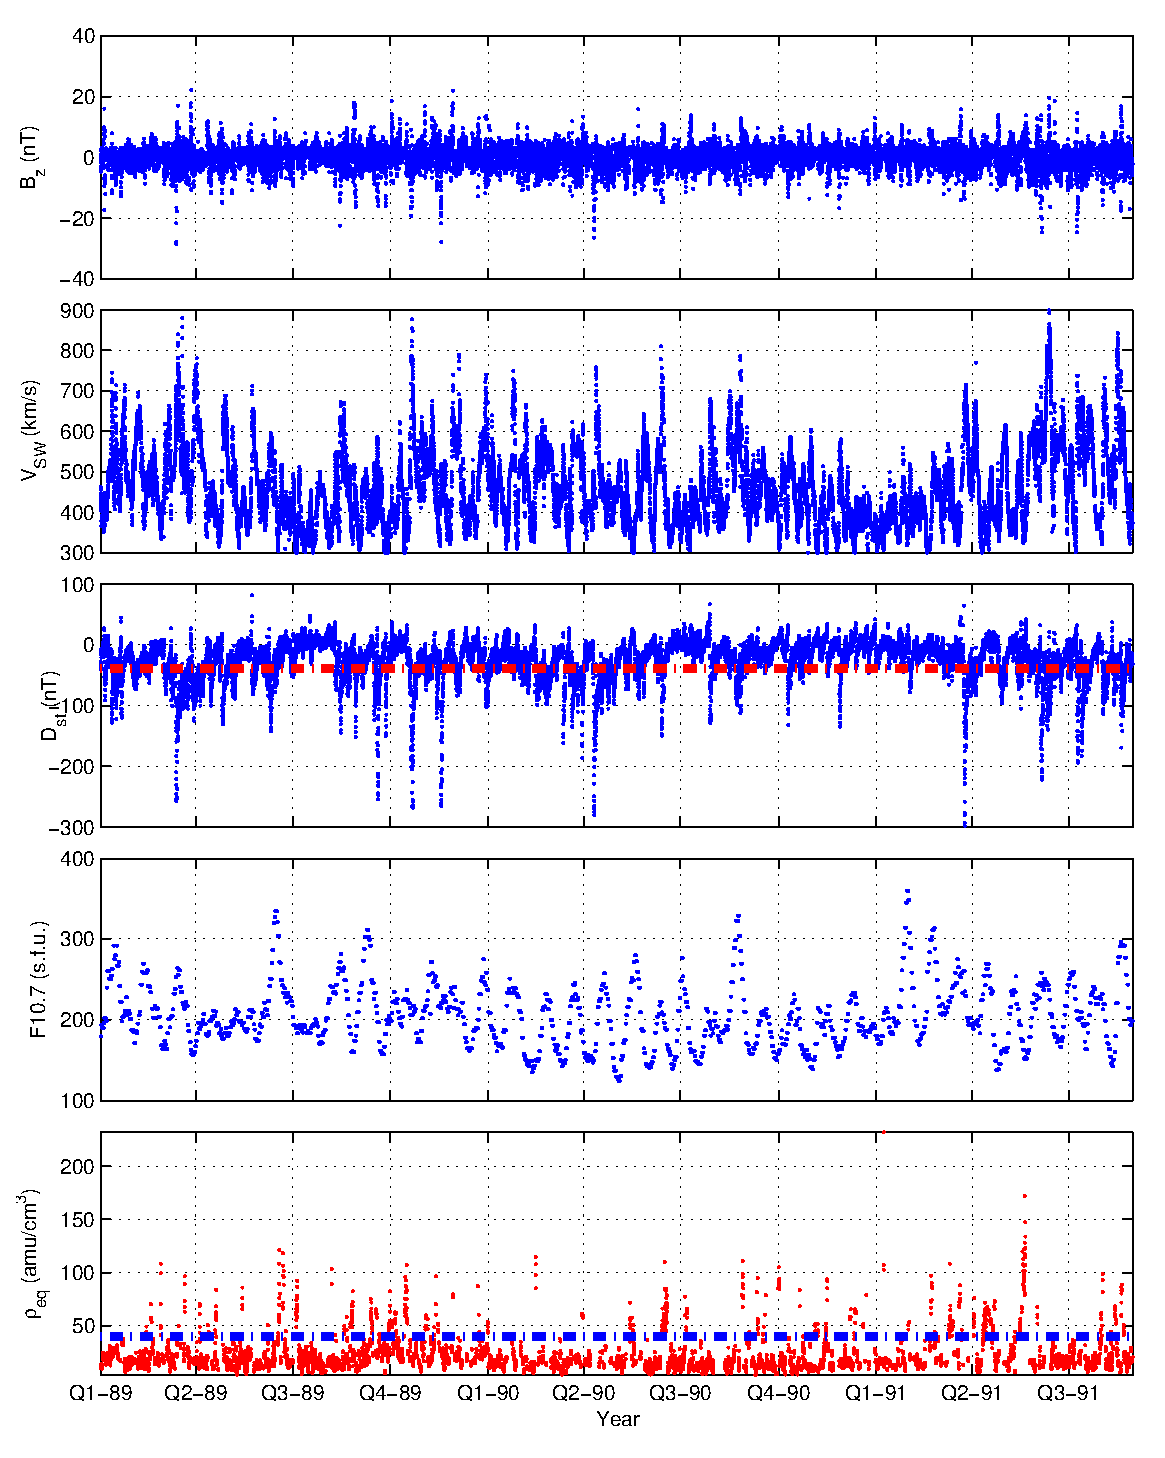
\includegraphics[scale=0.45]{paperfigures/alldata.eps}
\caption{Overview of data used in this study. The top four panels show parameters from \cite{Reconstruction} and the bottom panel is based on $\rho_{eq}$ from \cite{Denton} after interpolation and averaging described in the text. Dashed horizontal lines in the $D_{st}$ and $\rho_{eq}$ panels indicate sample event cutoff thresholds of $D_{st}=-50$~nT and $\rho_{eq}=40$~amu/cm$^3$}.
\label{AllData}
\end{figure}

\begin{figure}[htp!]
\centering
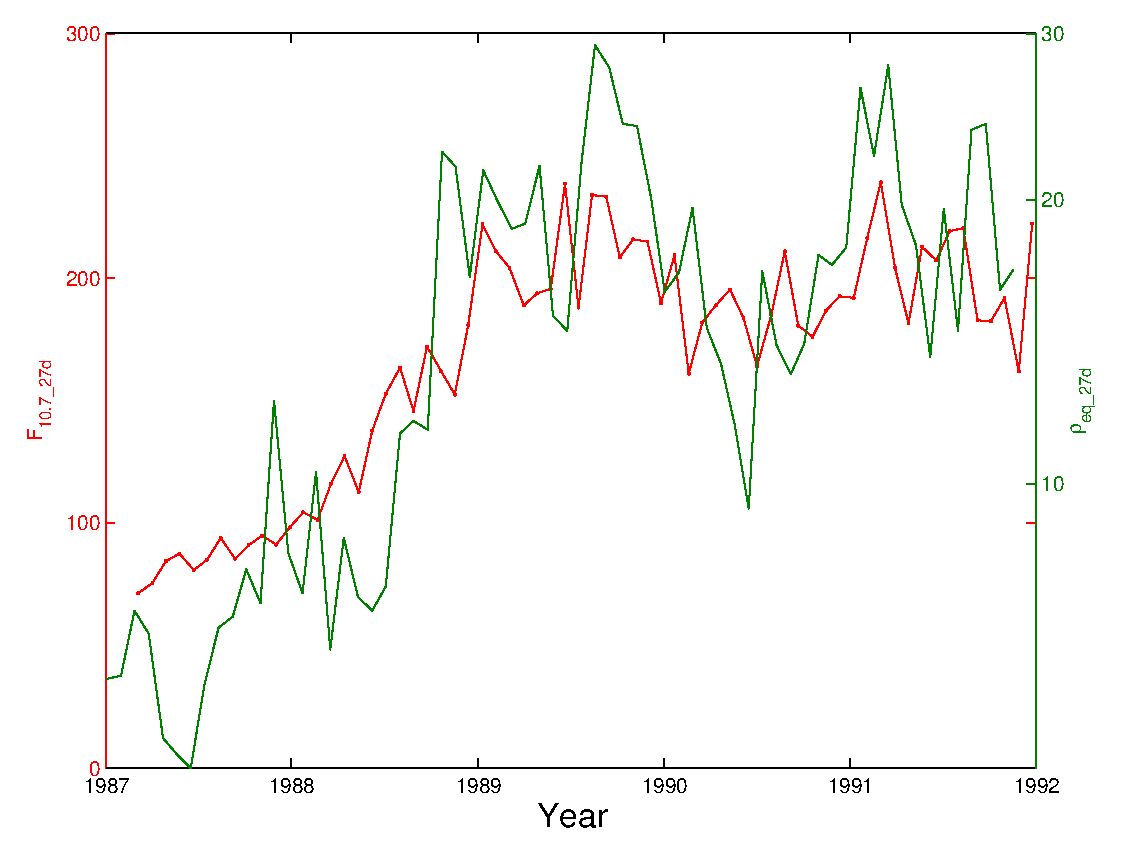
\includegraphics[scale=0.40]{paperfigures/F107MDAllData.eps}
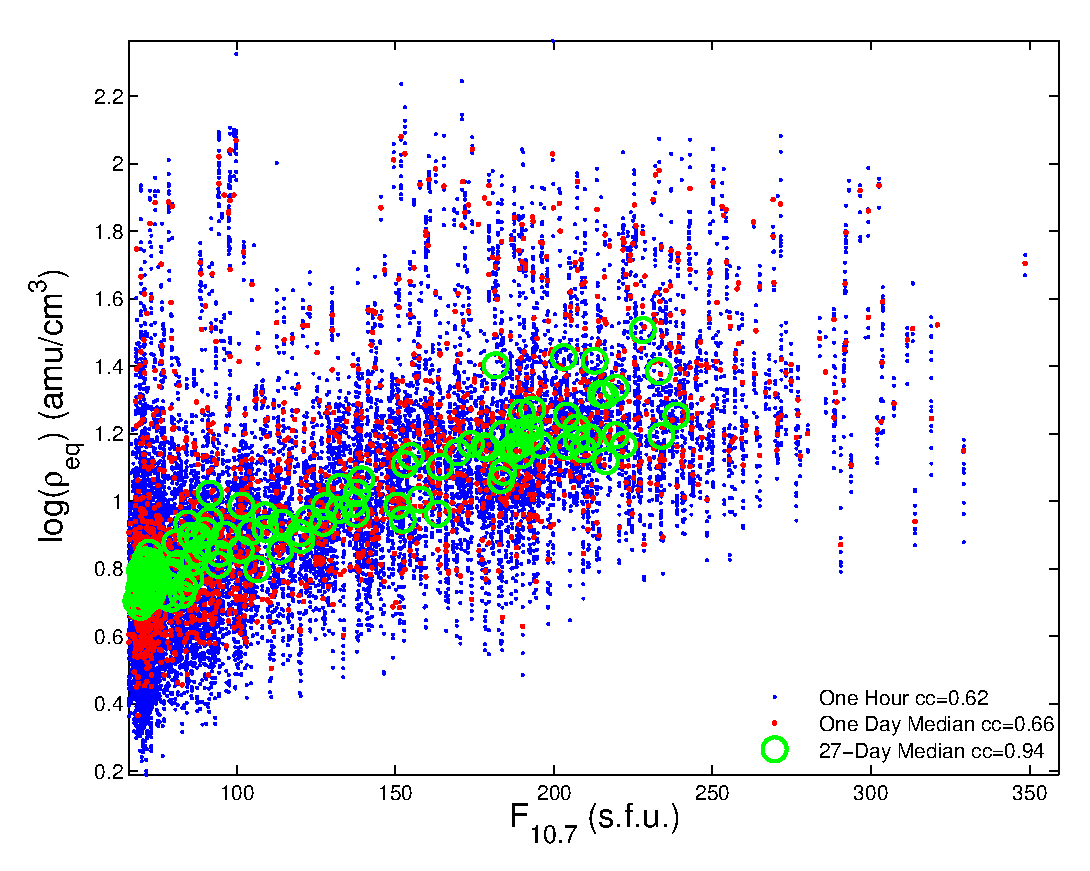
\includegraphics[scale=0.40]{paperfigures/ccplot.eps}
\caption{(a) 27-day averages of $F_{10.7}$ and $\rho_{eq}$. (b) Correlation between $\log(\rho_{eq})$ and $F_{10.7}$ using hour, day, and 27-day averaging intervals; compare to \cite{Takahashi2010} Fig.~14.}
\label{ccplot}
\end{figure}
\clearpage

\begin{figure}[tp!]
\centering
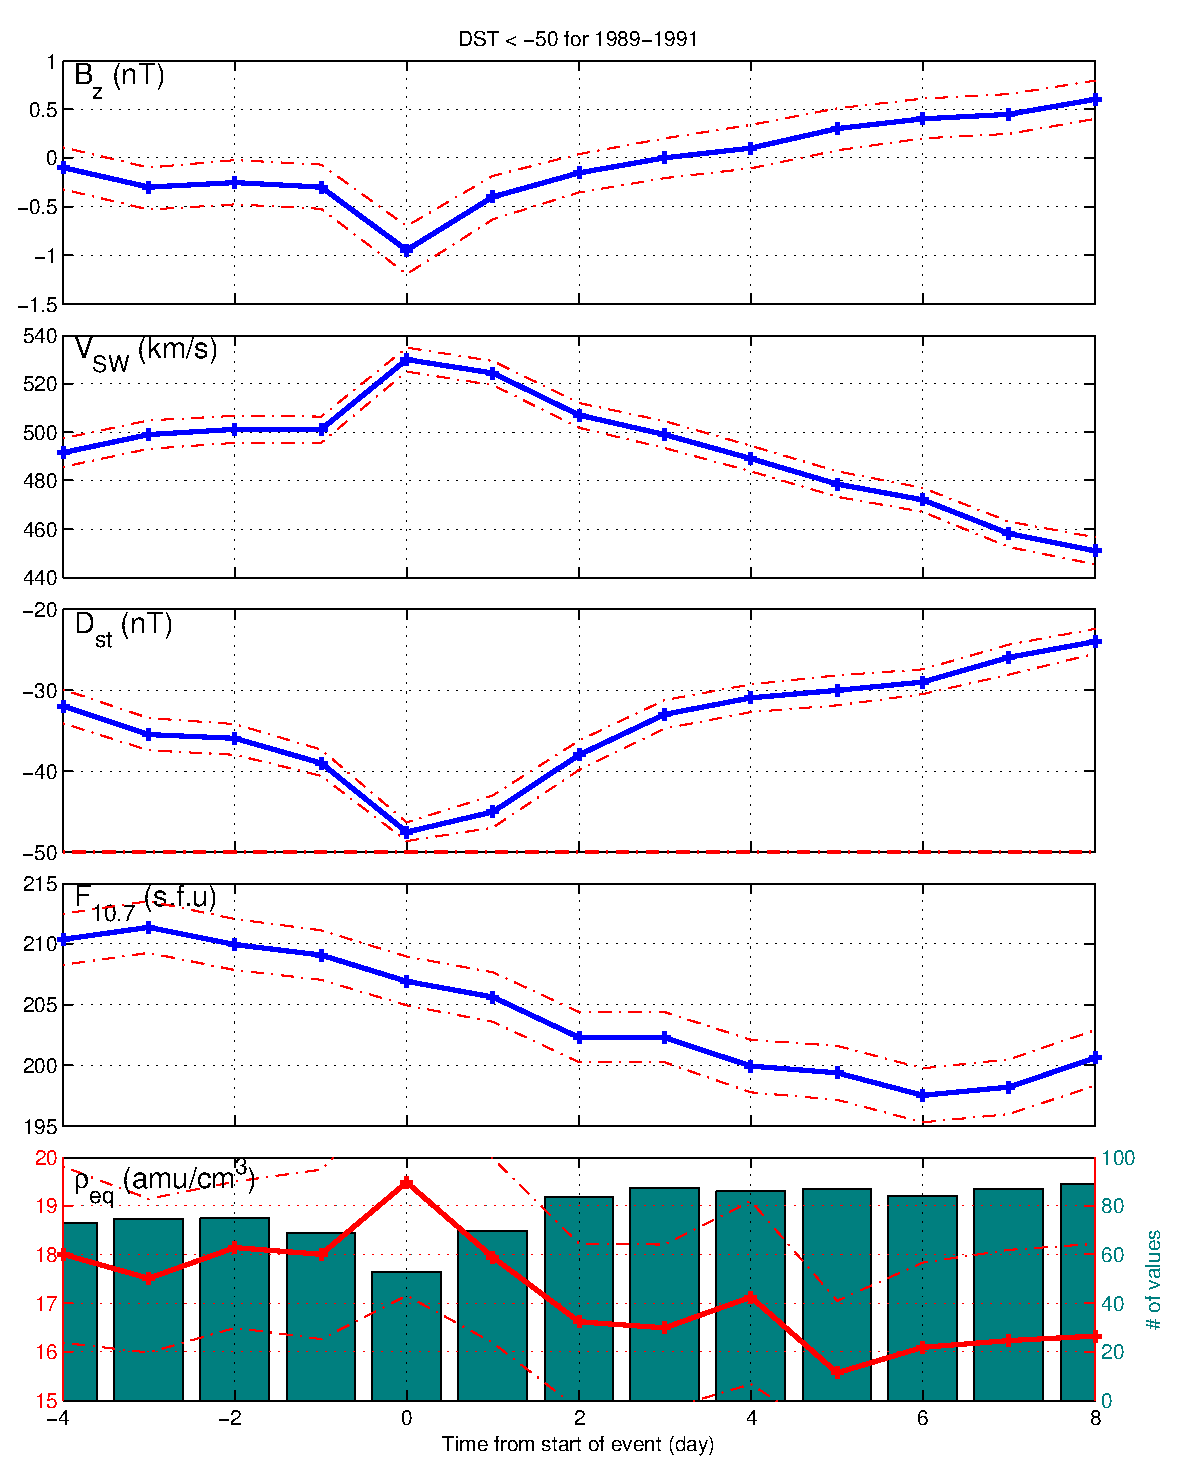
\includegraphics[scale=0.40]{paperfigures/stormavs-dst-50-tak.eps}
\rule[1ex]{5cm}{1pt}
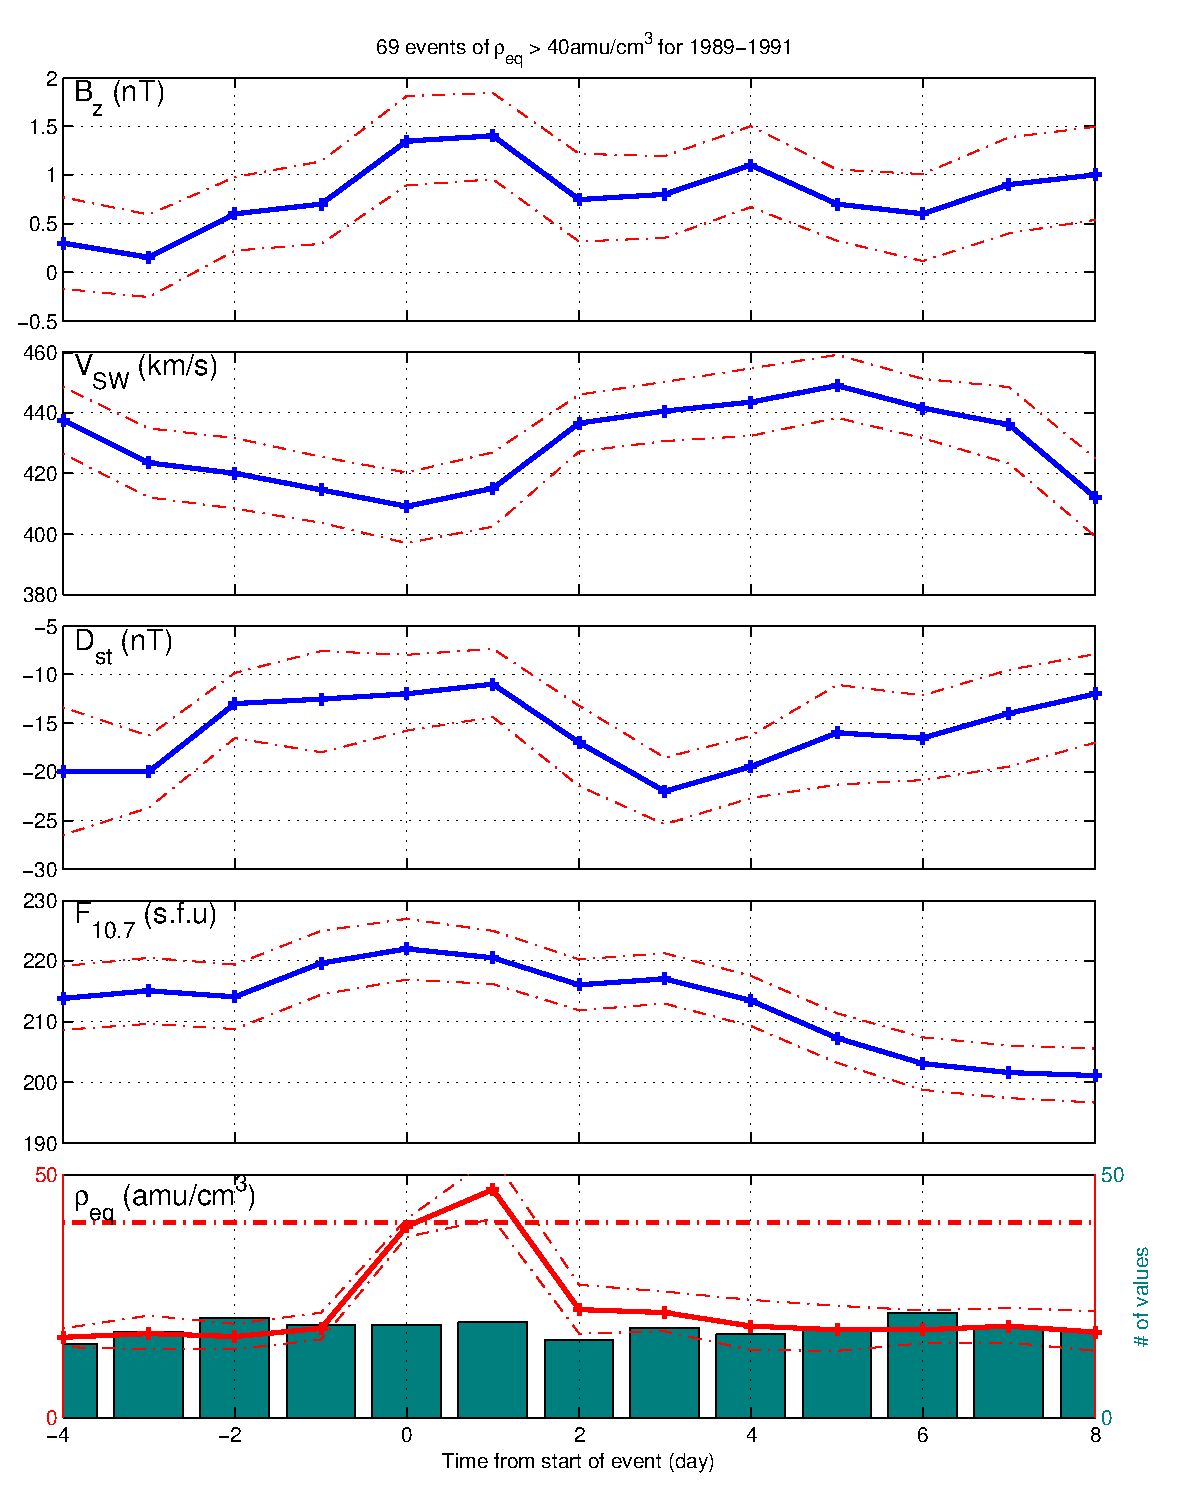
\includegraphics[scale=0.40]{paperfigures/stormavs-mass-tak.eps}
\caption{Events in the interval 1989-1991. Upper panel: $D_{st}$ events. Lower panel: $\rho_{eq}$ events.}
\label{DailyAverages}
\end{figure}

\begin{figure}[tp!]
\centering
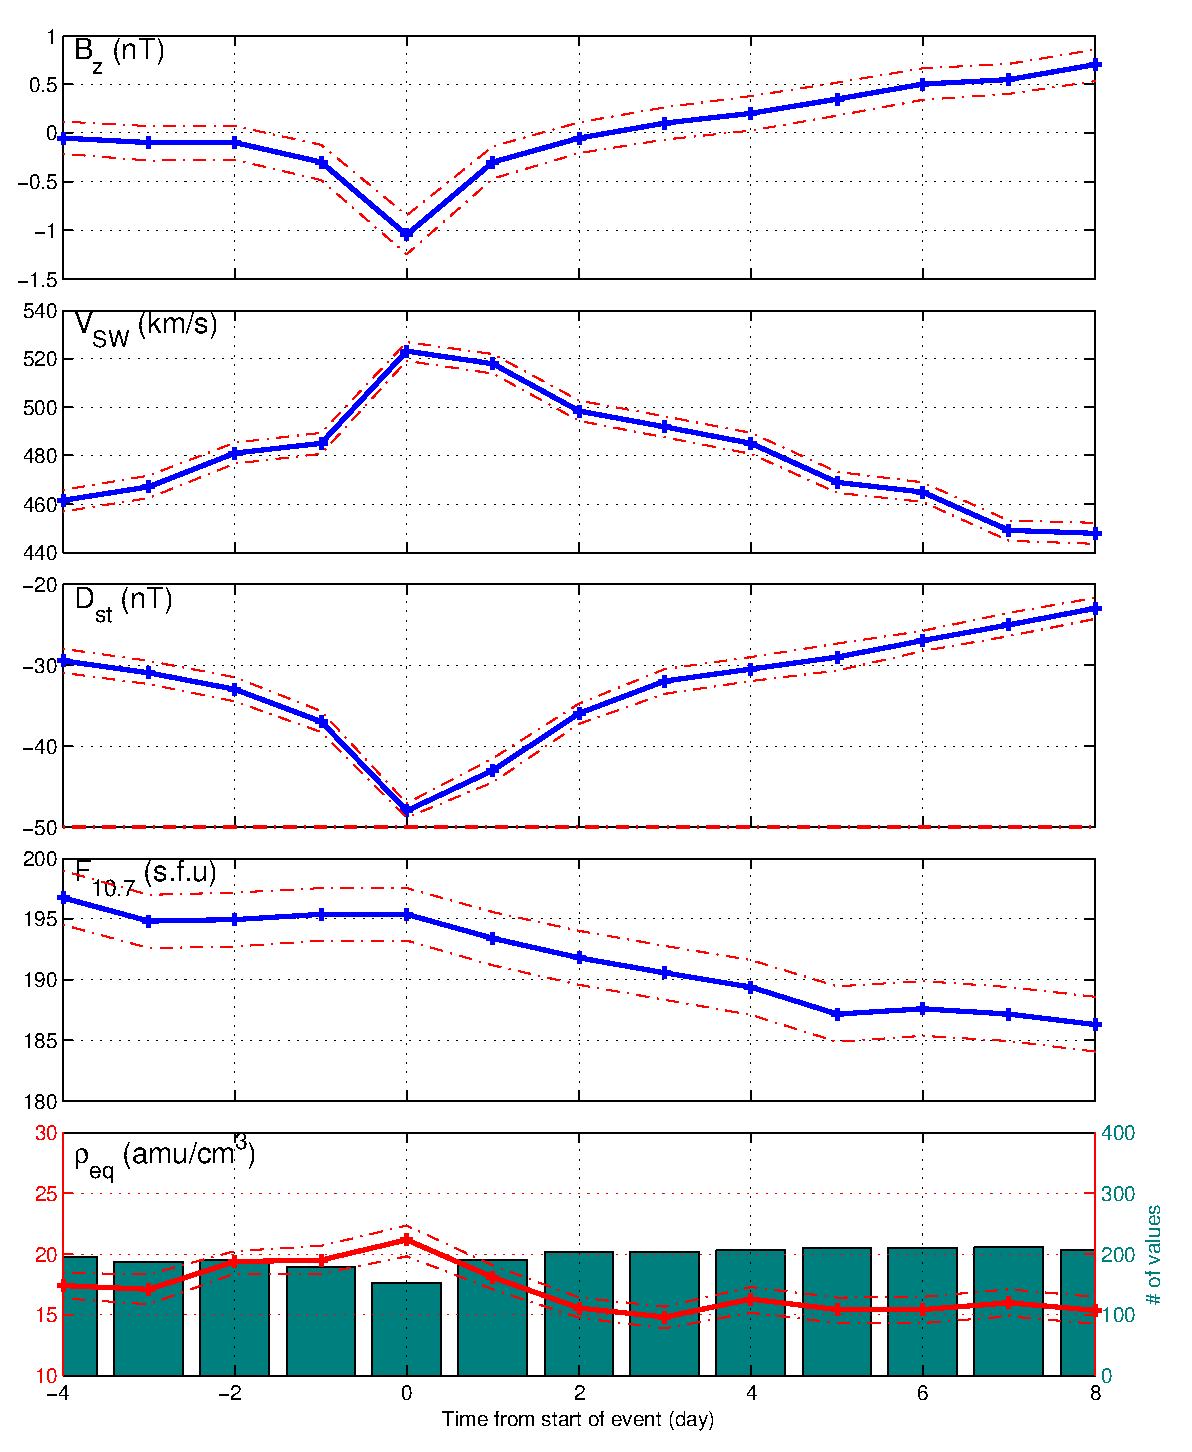
\includegraphics[scale=0.40]{paperfigures/stormavs-dst-day.eps}
\rule[1ex]{5cm}{1pt}
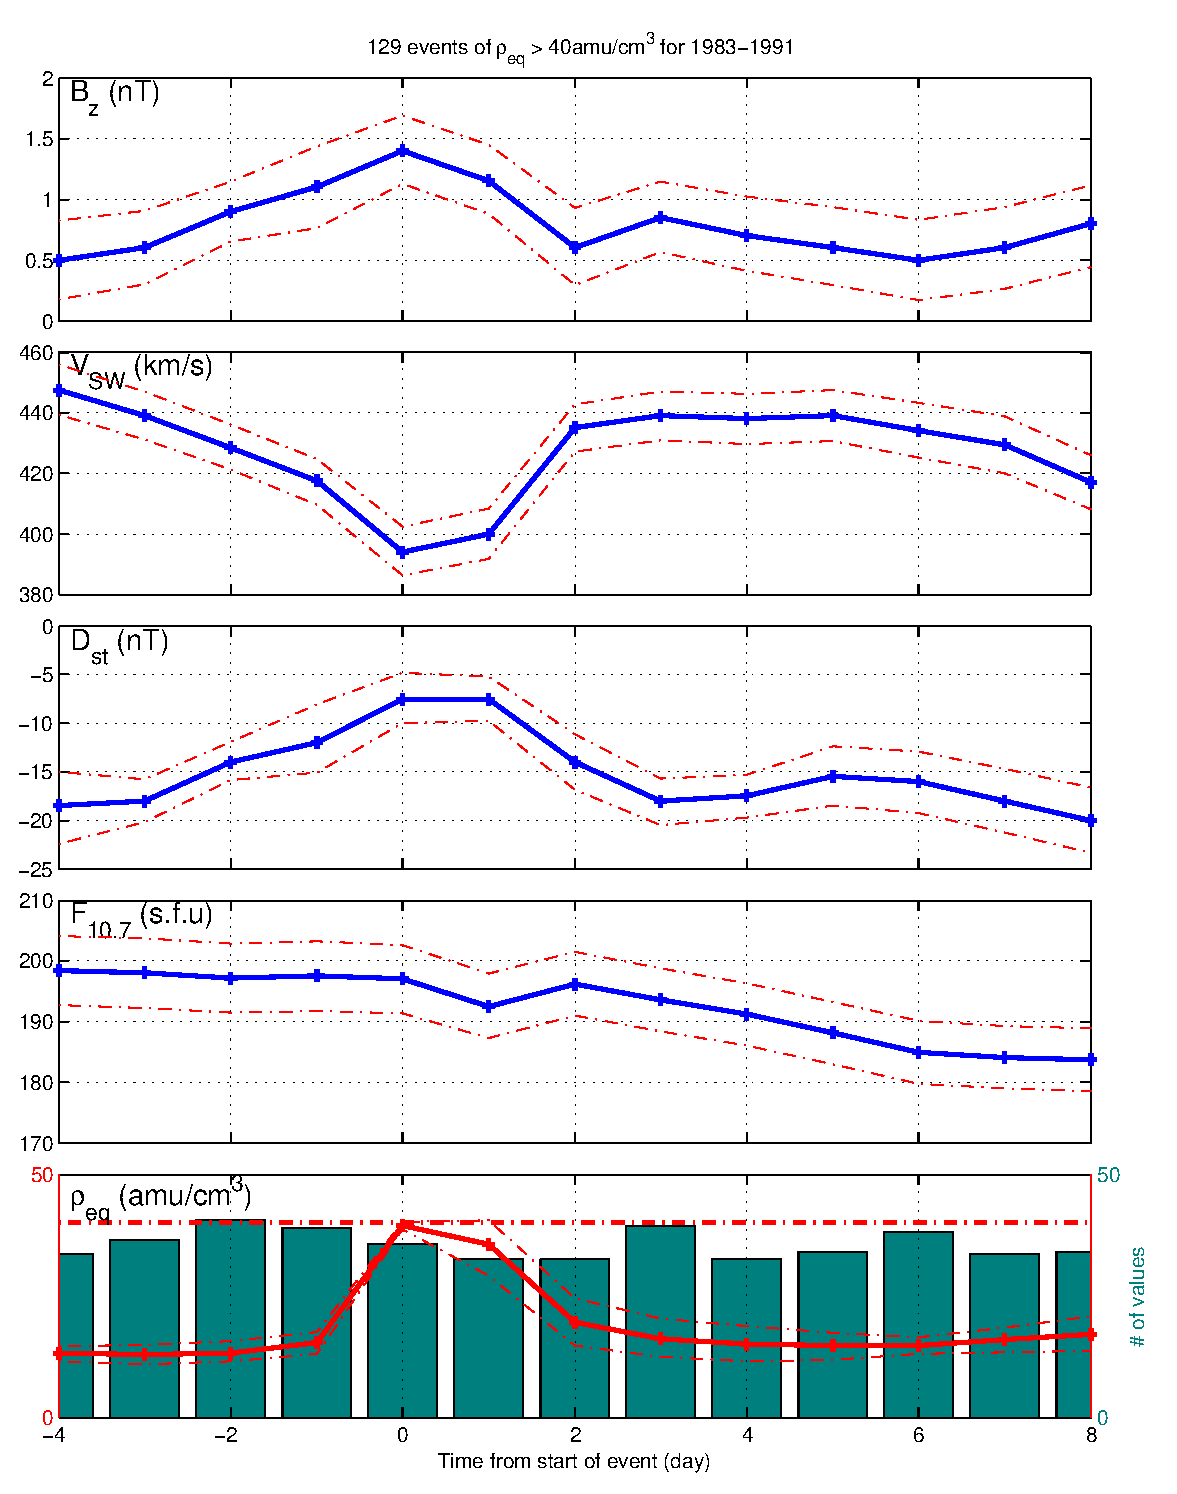
\includegraphics[scale=0.40]{paperfigures/stormavs-mass-day.eps}
\caption{Events in the interval 1983-1991.  Upper panel: $D_{st}$ events. Lower panel: $\rho_{eq}$ events.}
\label{DailyAveragesAllData}
\end{figure}
\clearpage

\begin{figure}[tp!]
\centering
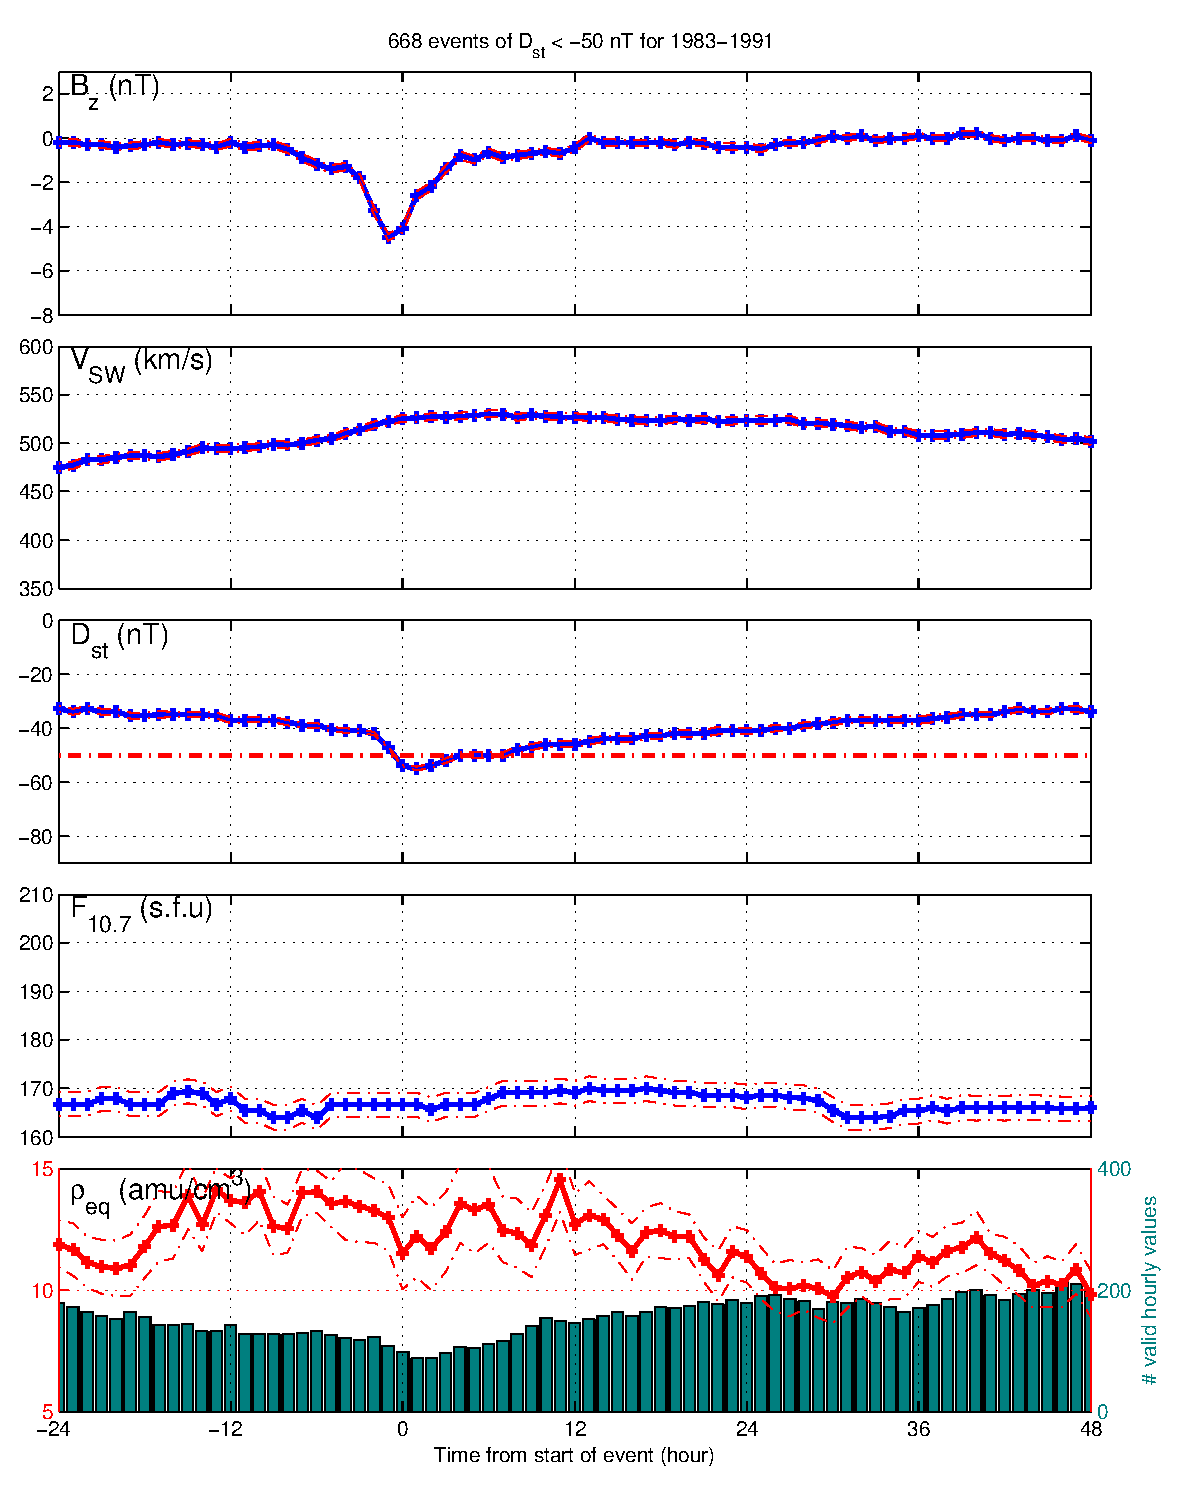
\includegraphics[scale=0.40]{paperfigures/stormavs-dst.eps}
\rule[1ex]{5cm}{1pt}
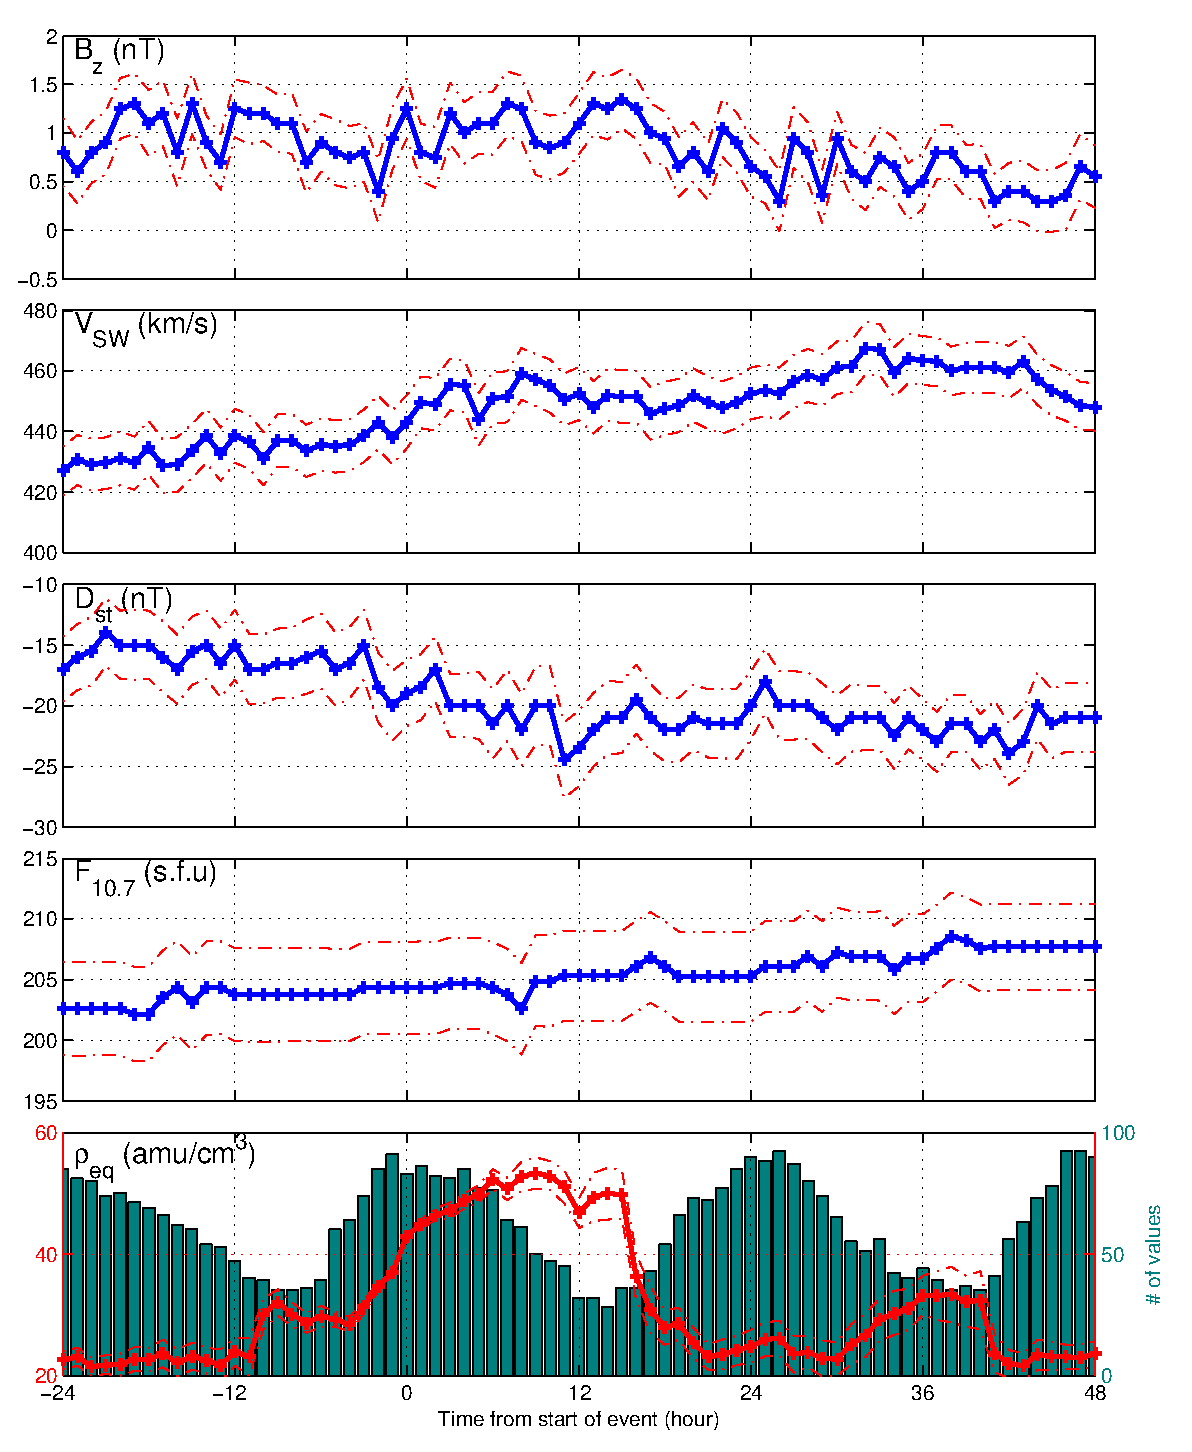
\includegraphics[scale=0.40]{paperfigures/stormavs-mass.eps}
\caption{(a) Average of solar wind and near-Earth measurements around the time $D_{st}$ crossed below $-50$~nT onset. (b) Same as (a) except around time intervals where mass density crossed above $40$~amu/cm$^3$.}
\label{Storms}
\end{figure}

\begin{figure}[tp!]
\centering
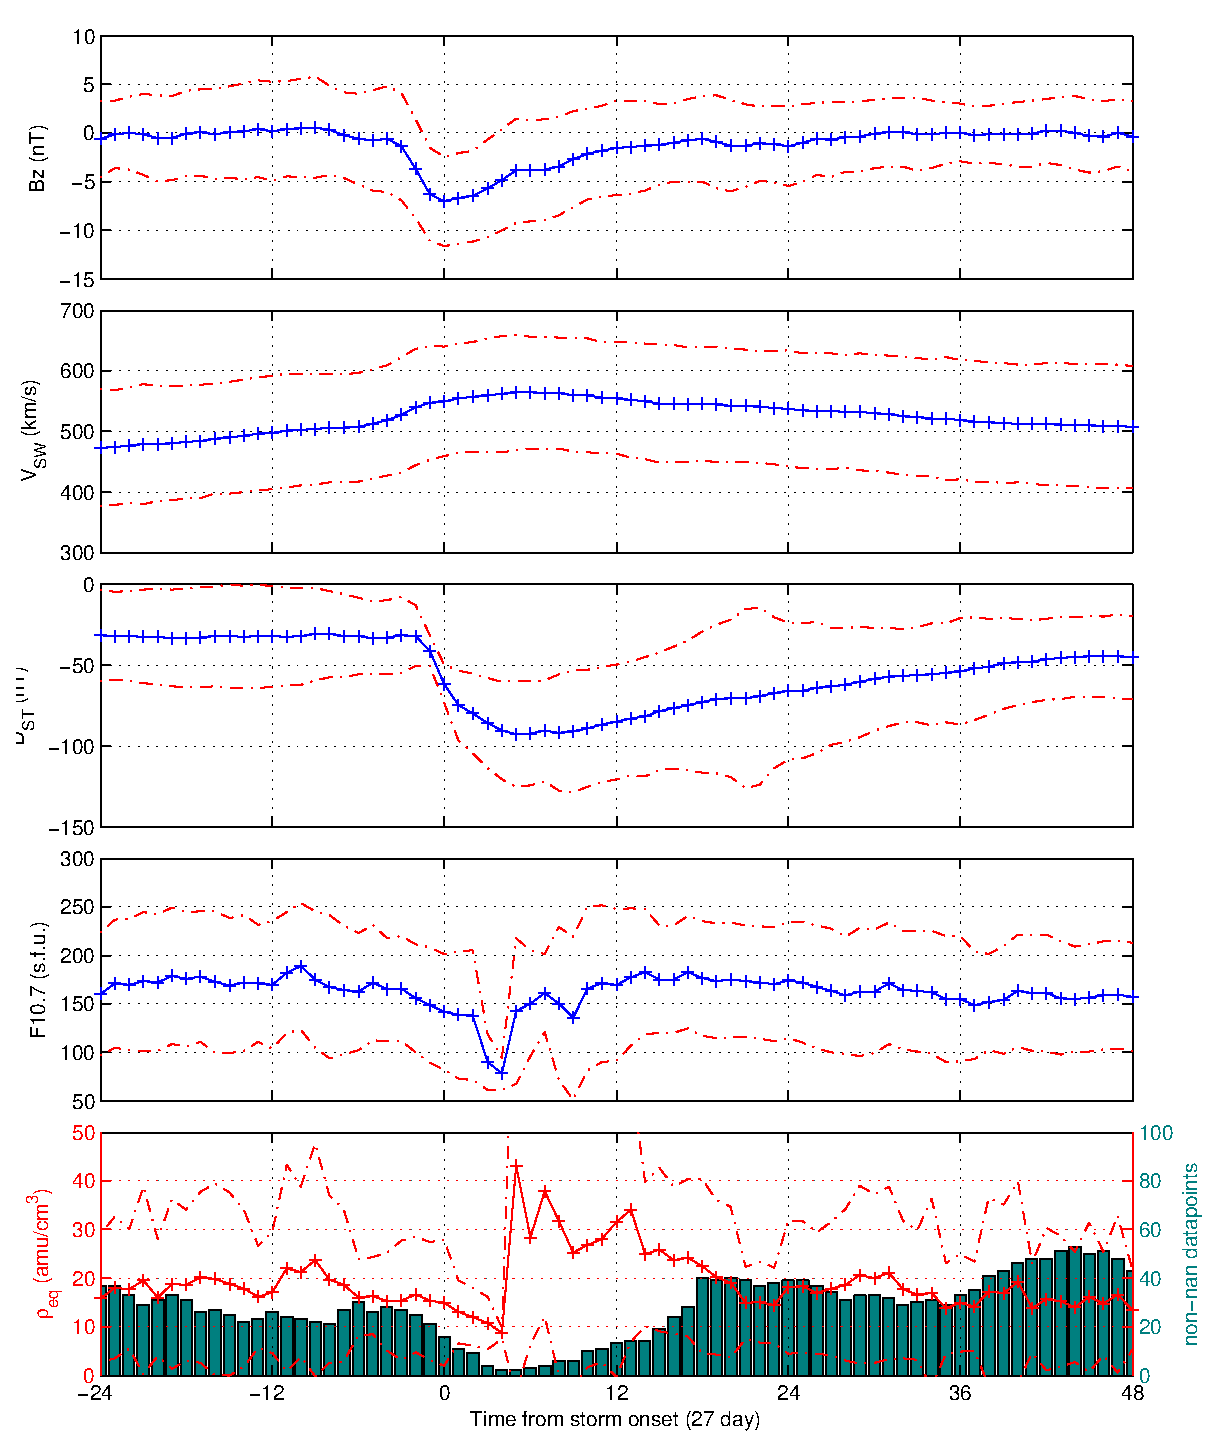
\includegraphics[scale=0.40]{paperfigures/stormavs-dd12.eps}
\rule[1ex]{5cm}{1pt}
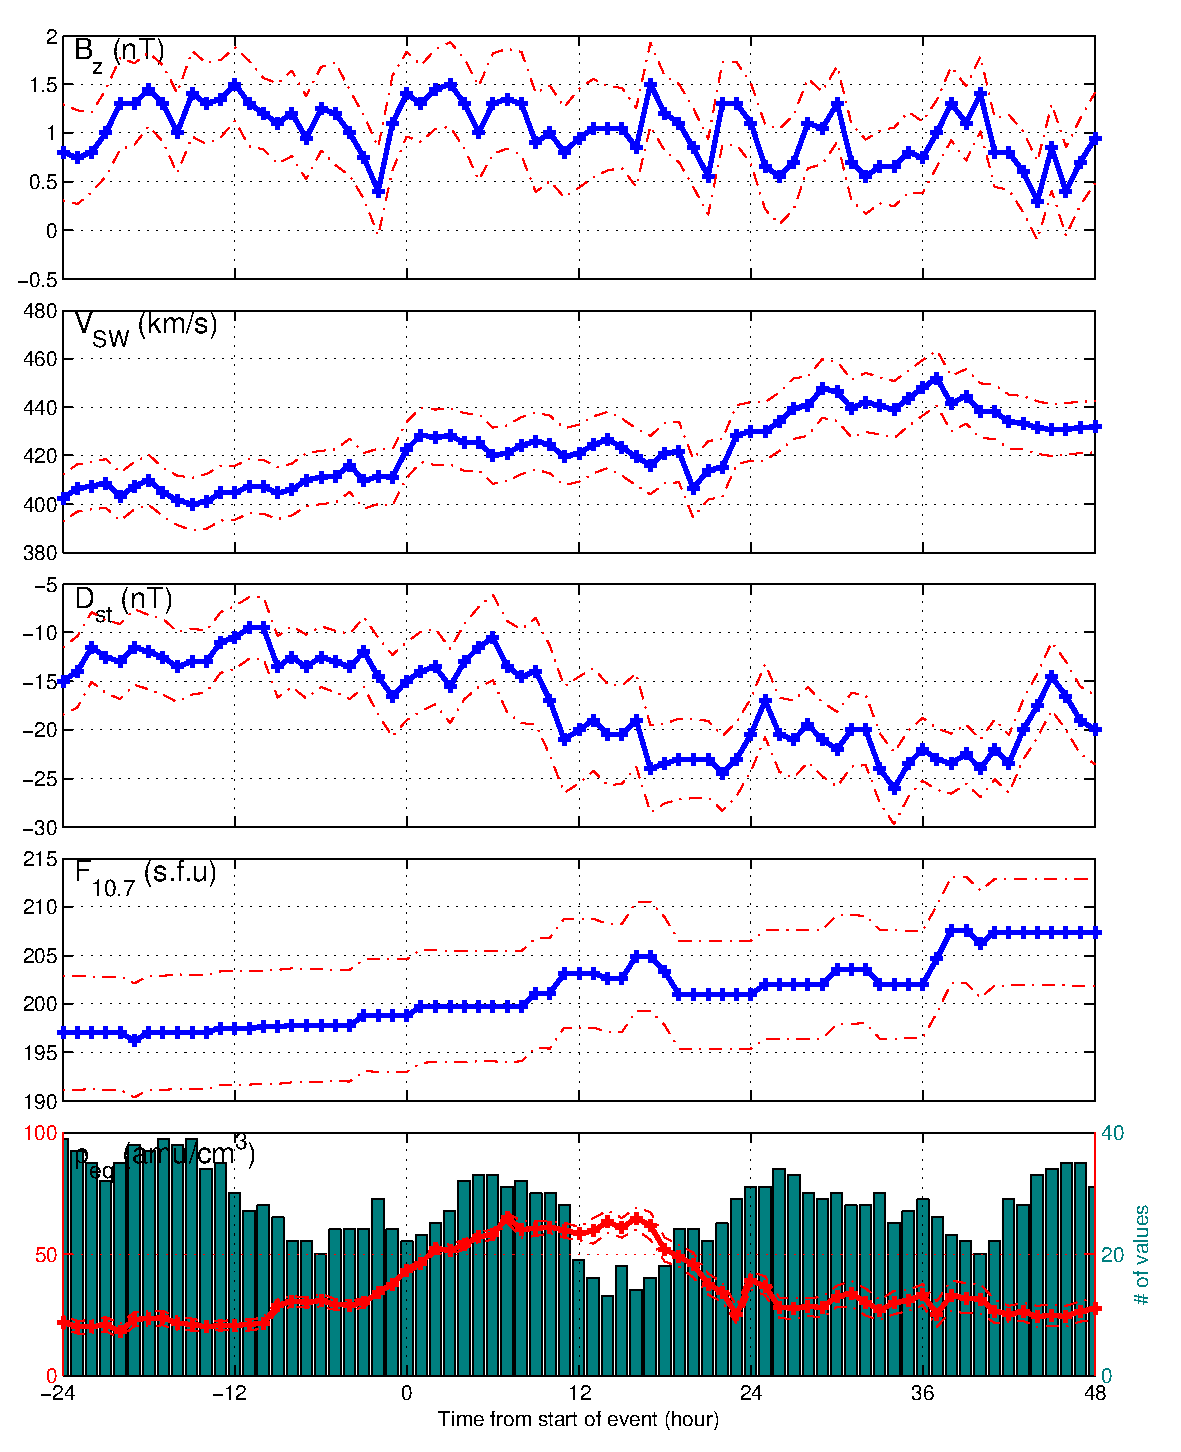
\includegraphics[scale=0.40]{paperfigures/stormavs-md12.eps}
\caption{(a) Same as Figure \ref{Storms}(a) except with constraint that $D_{st}$ stayed below $-50$~nT for at least 12~hours. (b) Same as Figure \ref{Storms}(b) except for constrain that $\rho_{eq}$ stayed above $50$~amu/cm$^3$ for at least 12 hours.}
\label{Mspec}
\end{figure}
\clearpage

\begin{figure}[tp!]
\centering
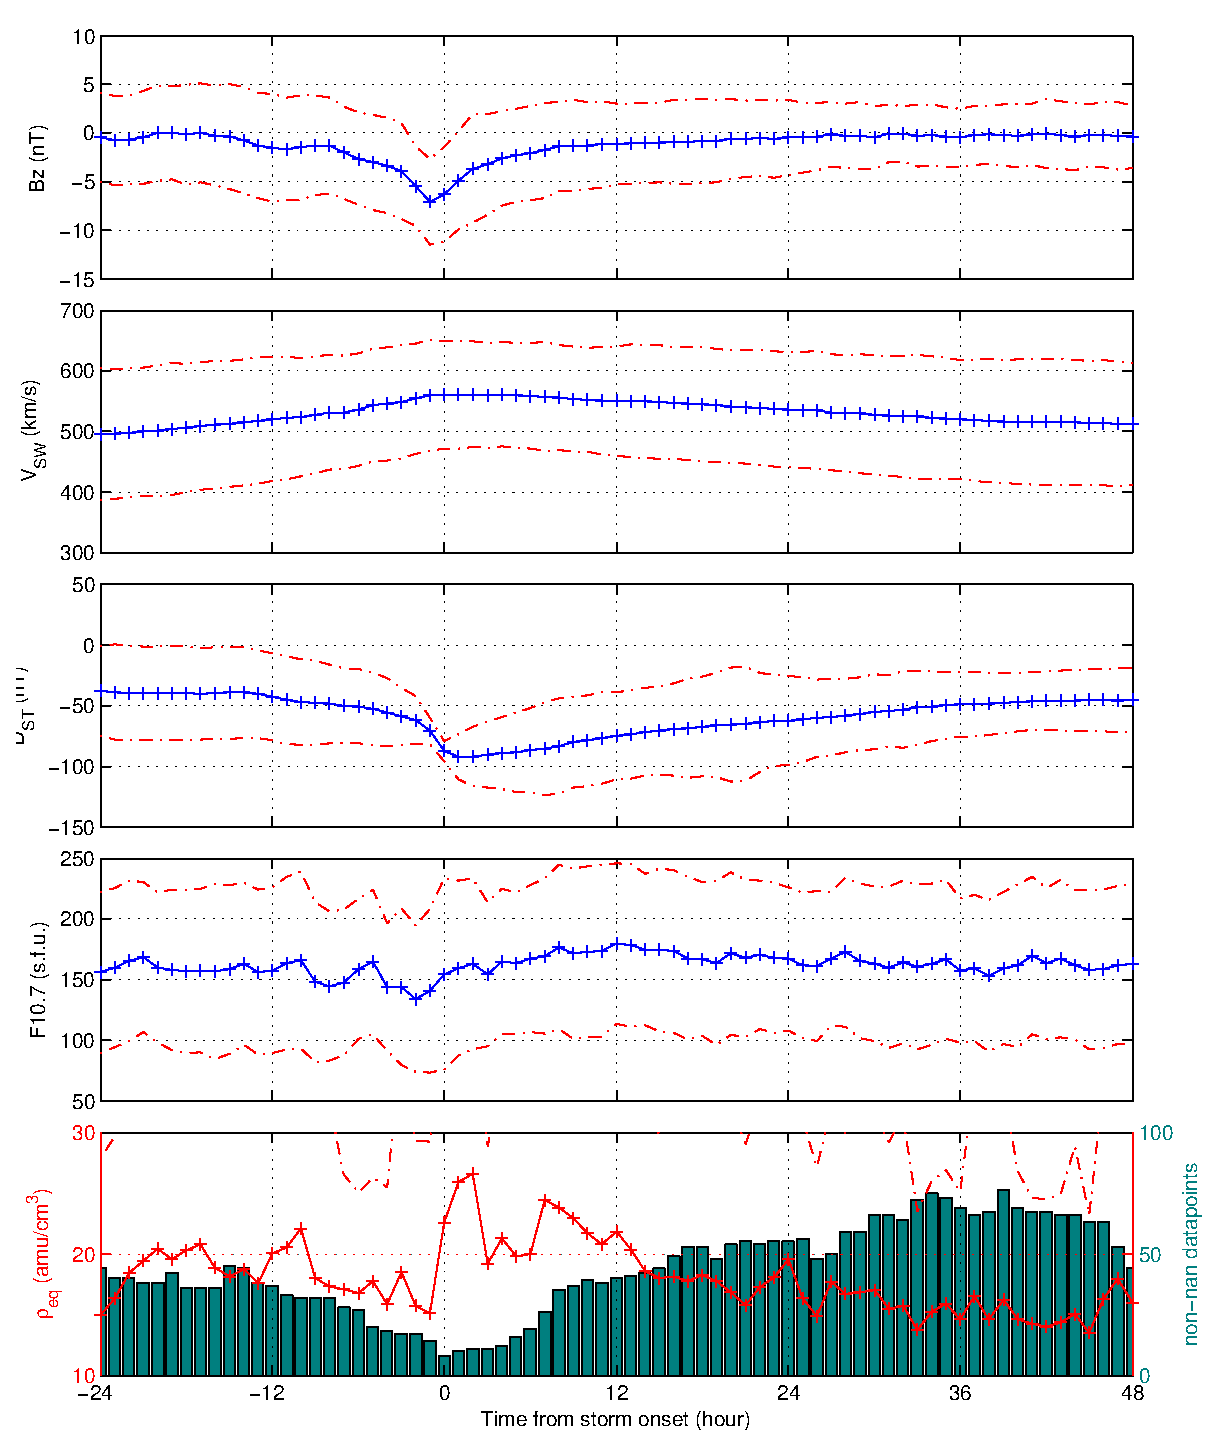
\includegraphics[scale=0.40]{paperfigures/stormavs-d80.eps}
\rule[1ex]{5cm}{1pt}
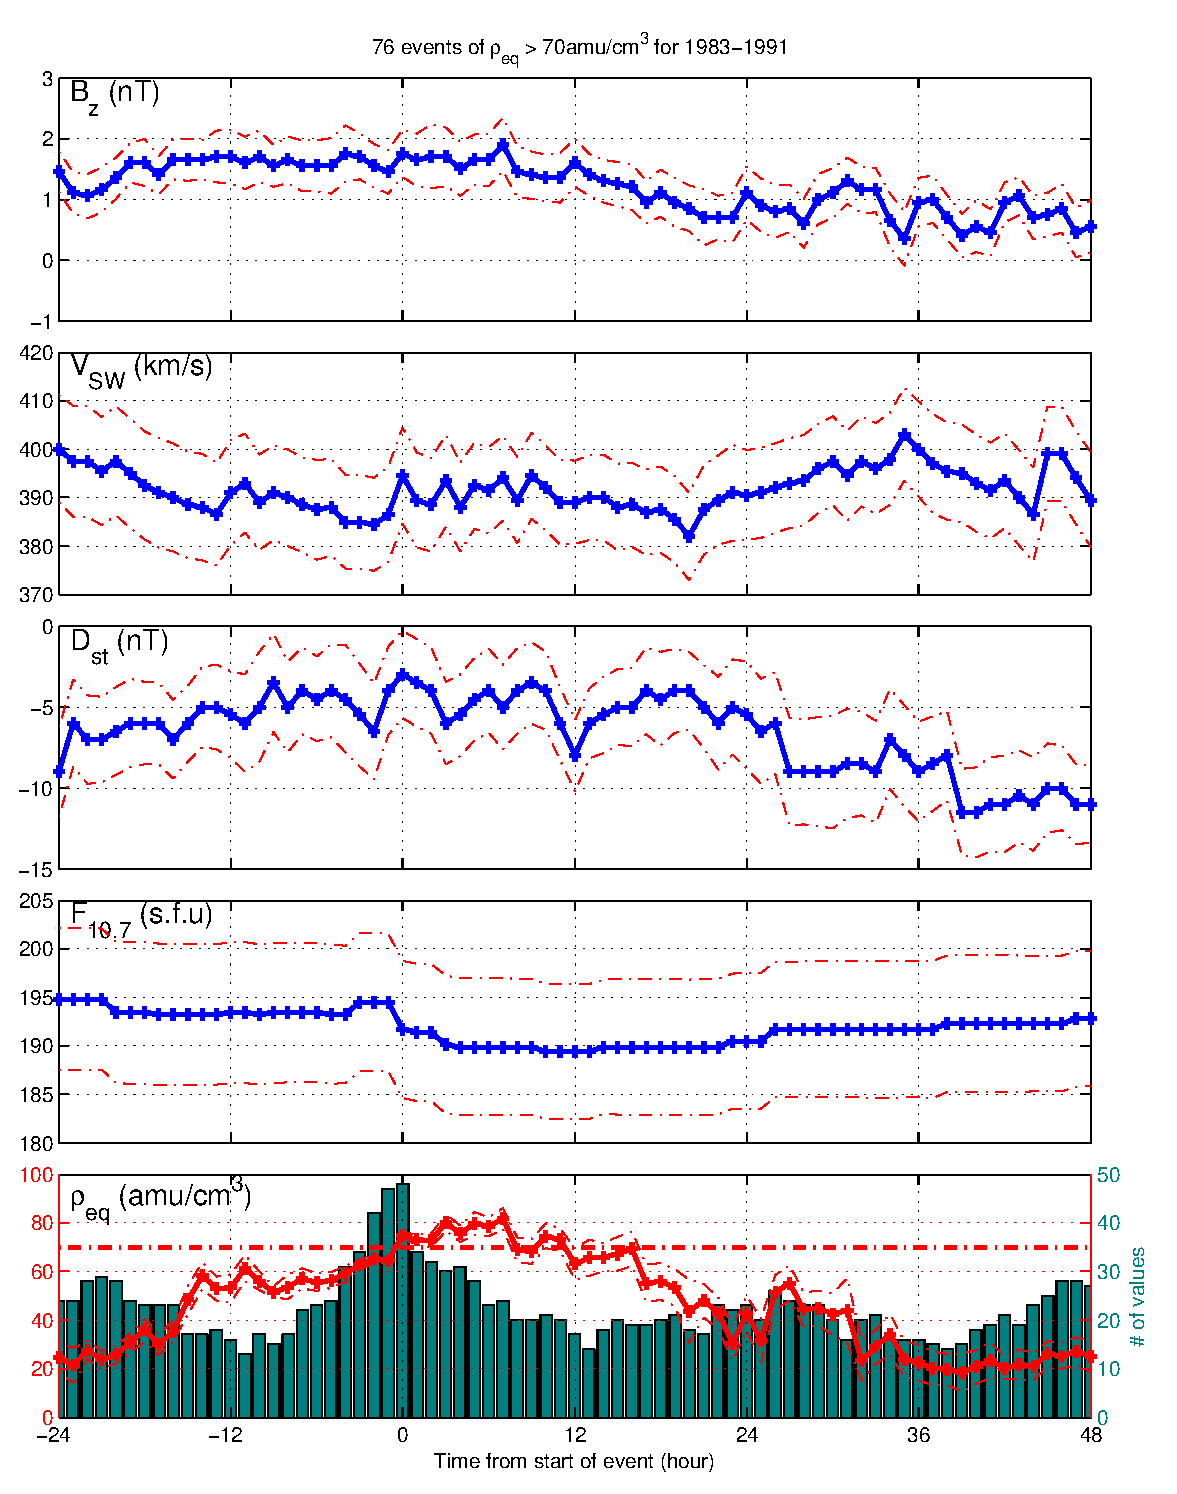
\includegraphics[scale=0.40]{paperfigures/stormavs-m70.eps}
\caption{(a) Same as Figure \ref{Storms}(a) except with constraint that $D_{st}$ crossed below $-80$~nT (b) Same as Figure \ref{Storms}(b) except for constrain that $\rho_{eq}$ crossed above $70$~amu/cm$^3$.}
\label{Dspec}
\end{figure}

\begin{figure}[tp!]
\centering
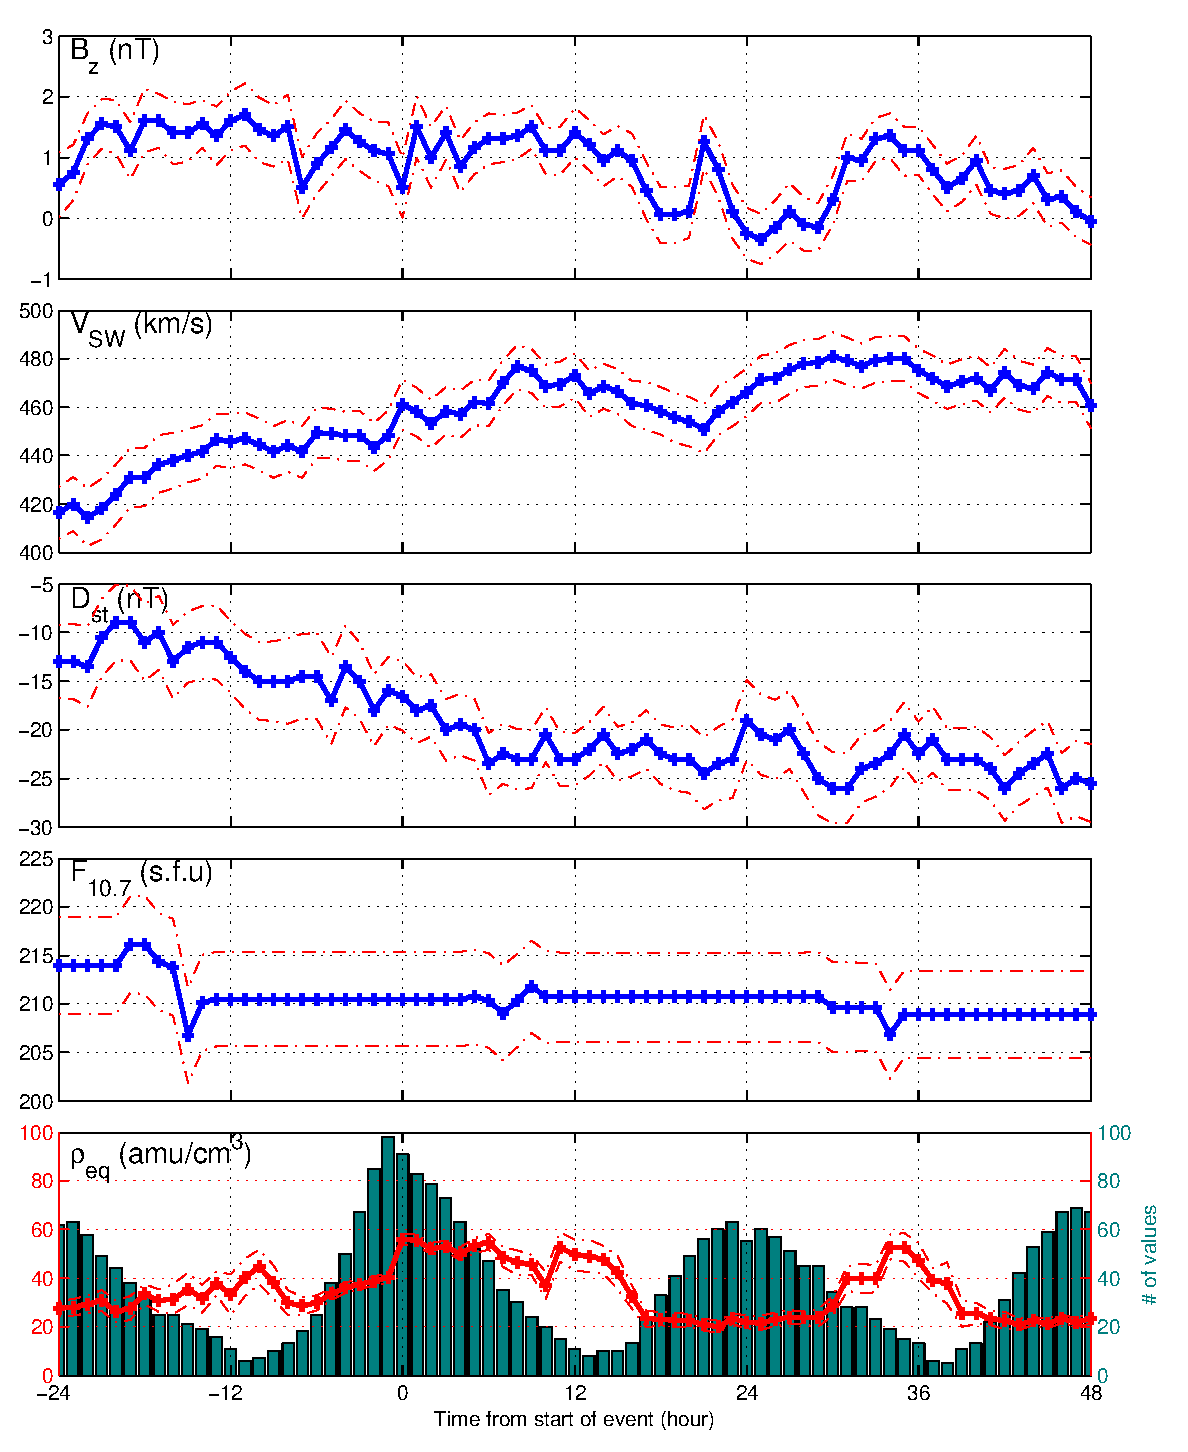
\includegraphics[scale=0.40]{paperfigures/stormavs-diffden-10amu.eps}
\rule[1ex]{5cm}{1pt}
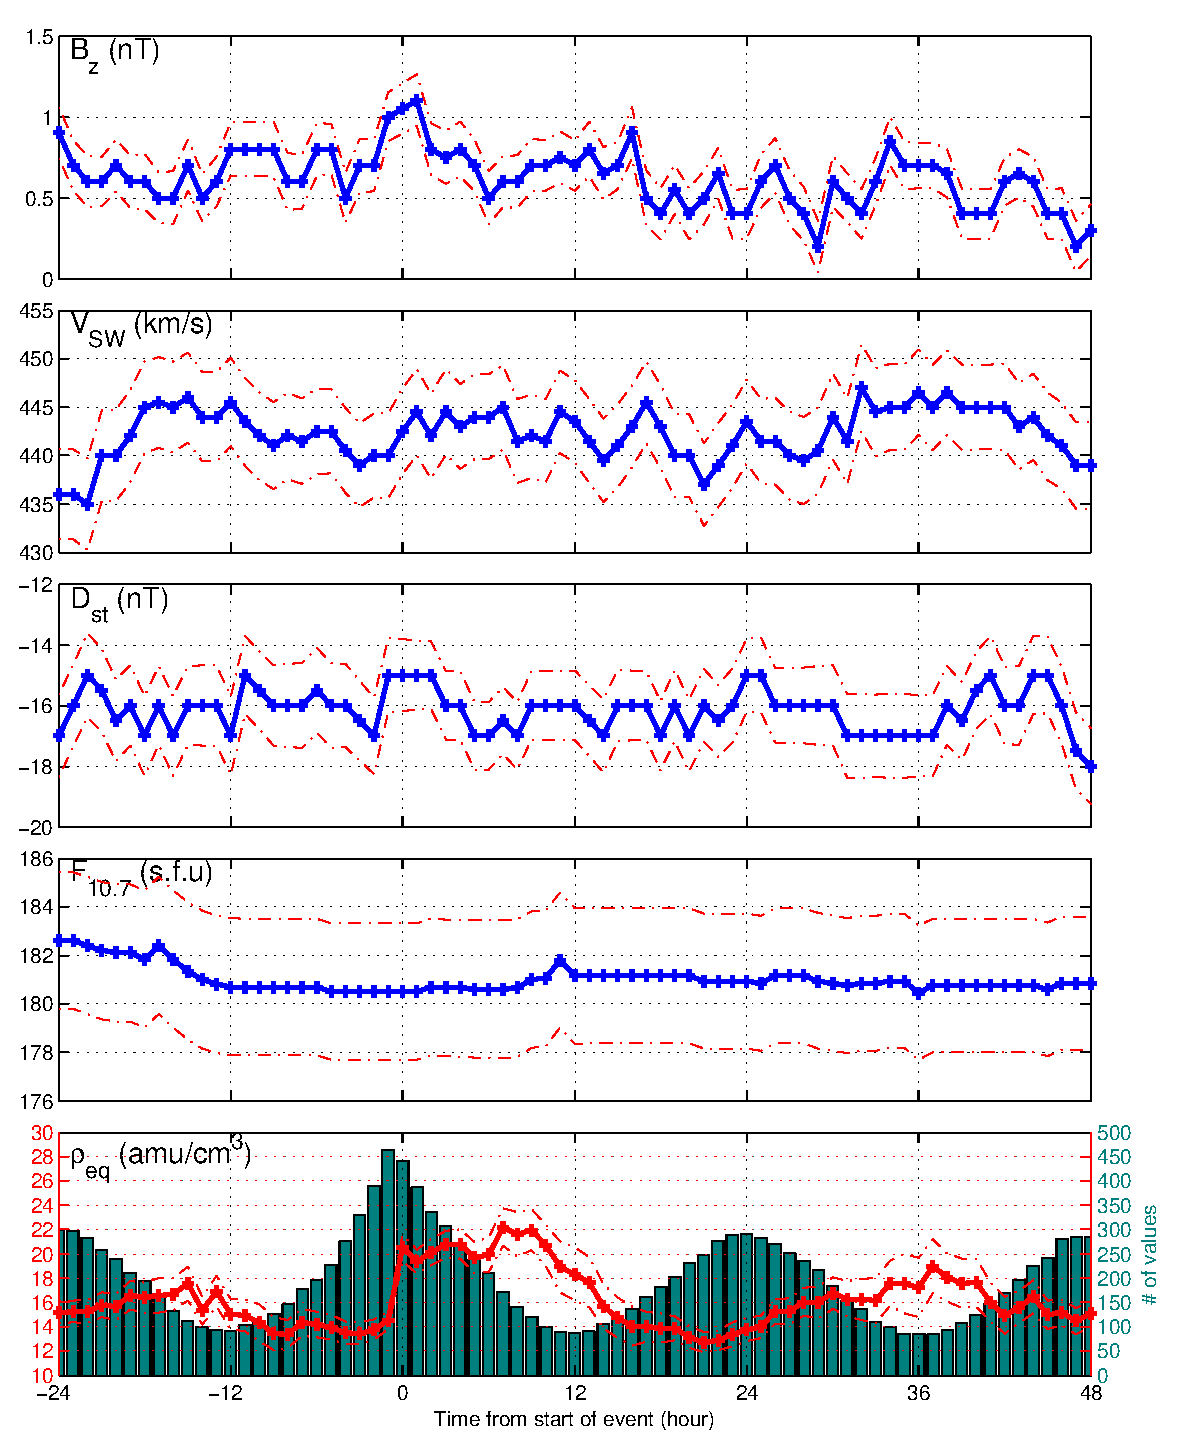
\includegraphics[scale=0.40]{paperfigures/stormavs-diffden-30percent.eps}
\caption{(a) diff($\rho_{eq}$) $>$ 10$\frac{amu}{hour}$. (b) diff($\rho_{eq}$) $>$ 30$\frac{\%}{hour}$}
\label{rhochange}
\end{figure}
\clearpage

\begin{figure}[tp!]
\centering
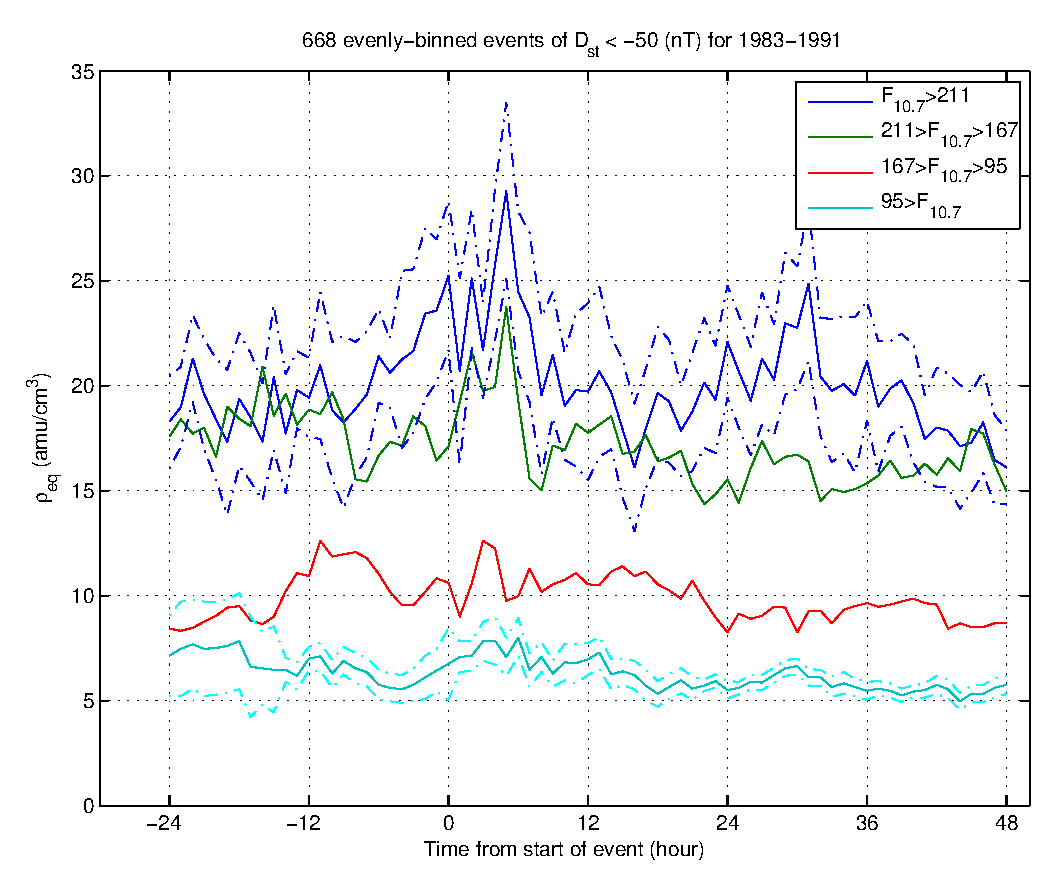
\includegraphics[scale=0.40]{paperfigures/HighLowF107rhoeq.eps}
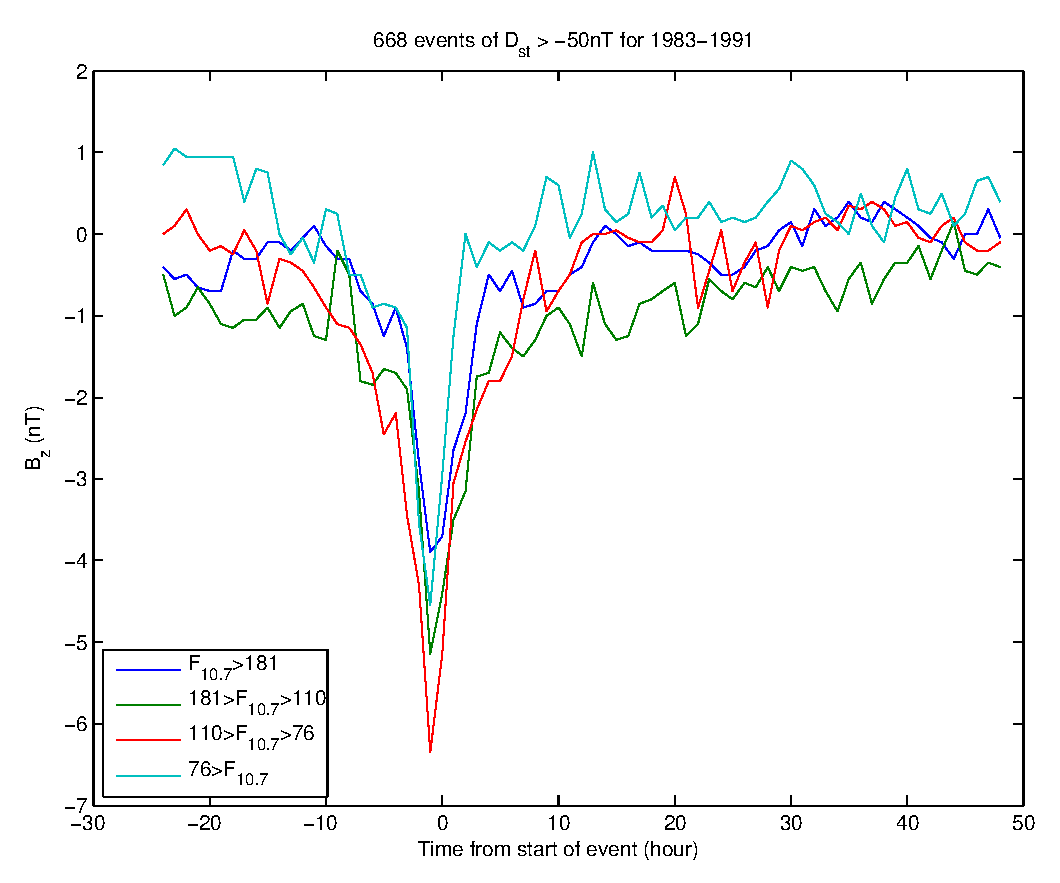
\includegraphics[scale=0.40]{paperfigures/HighLowF107Bz.eps}
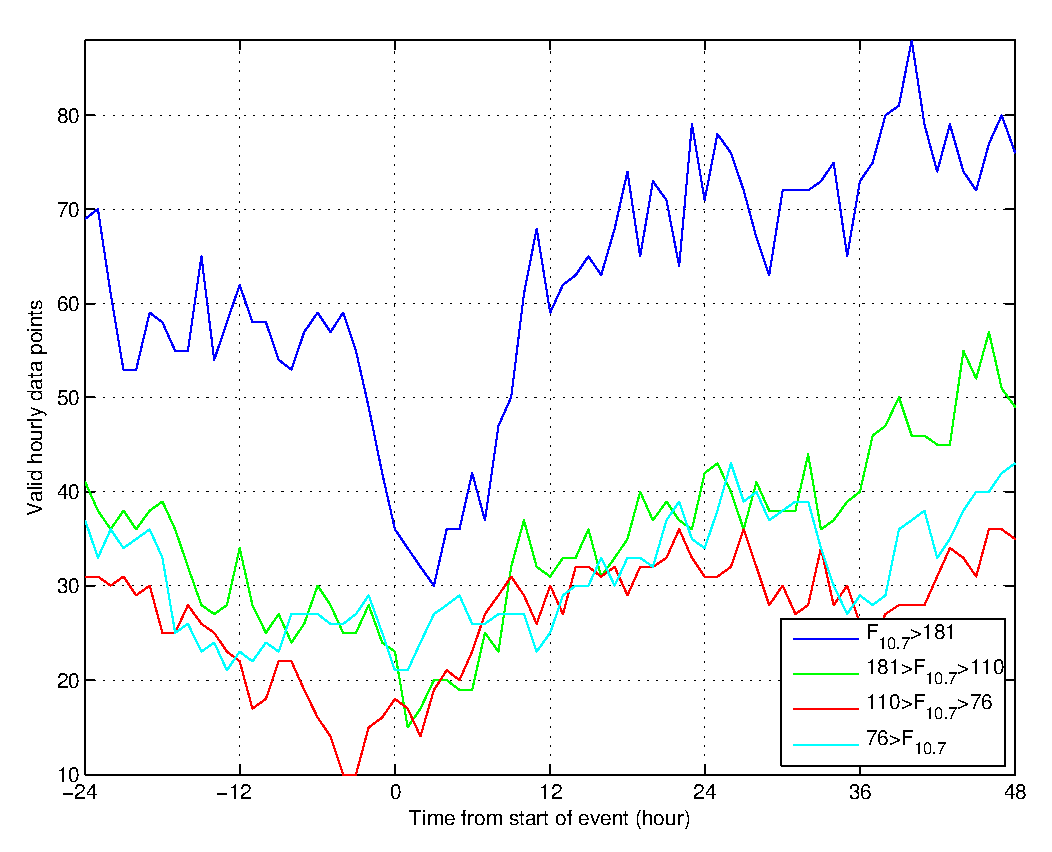
\includegraphics[scale=0.40]{paperfigures/HighLowF107valid.eps}
\caption{Binning events by $F_{10.7}$ value at onset for $\rho_{eq}$ and, in the middle panel, $B_z$. Lower panel shows number of valid points in each bin}
\label{f107bin}
\end{figure}

\begin{figure}[tp]
\centering
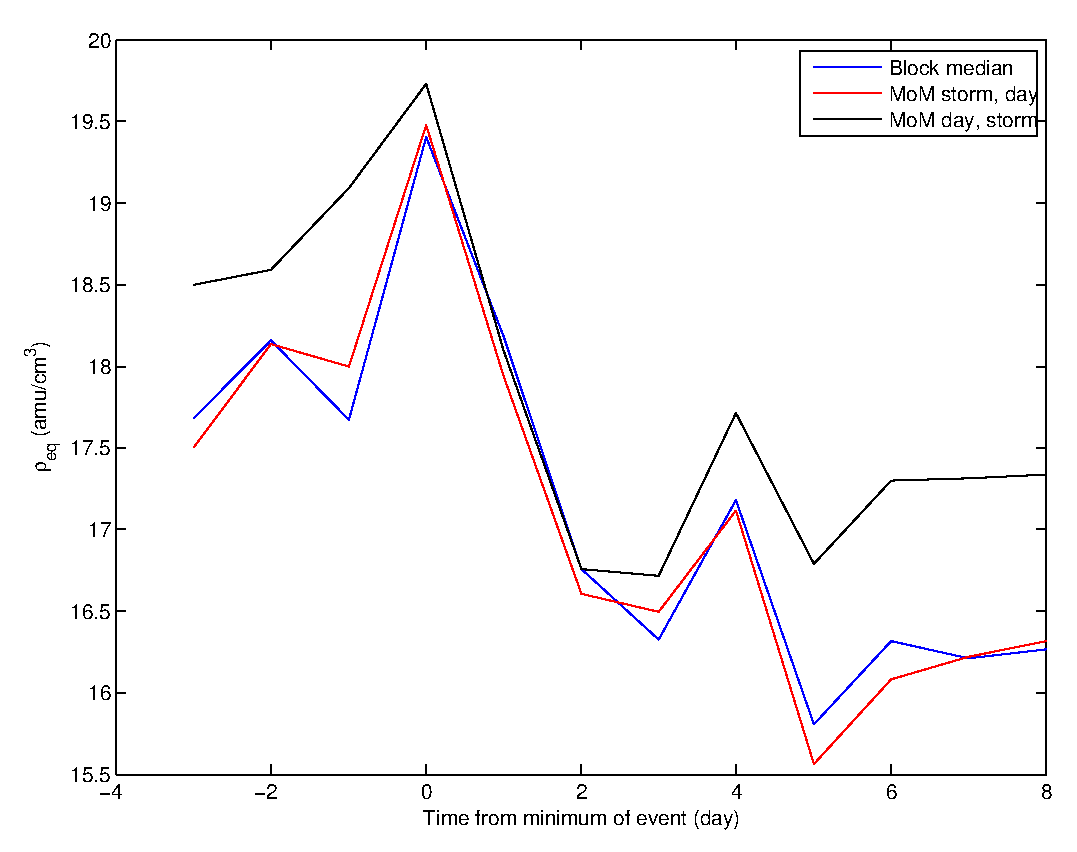
\includegraphics[scale=0.40]{paperfigures/blockmedian.eps}
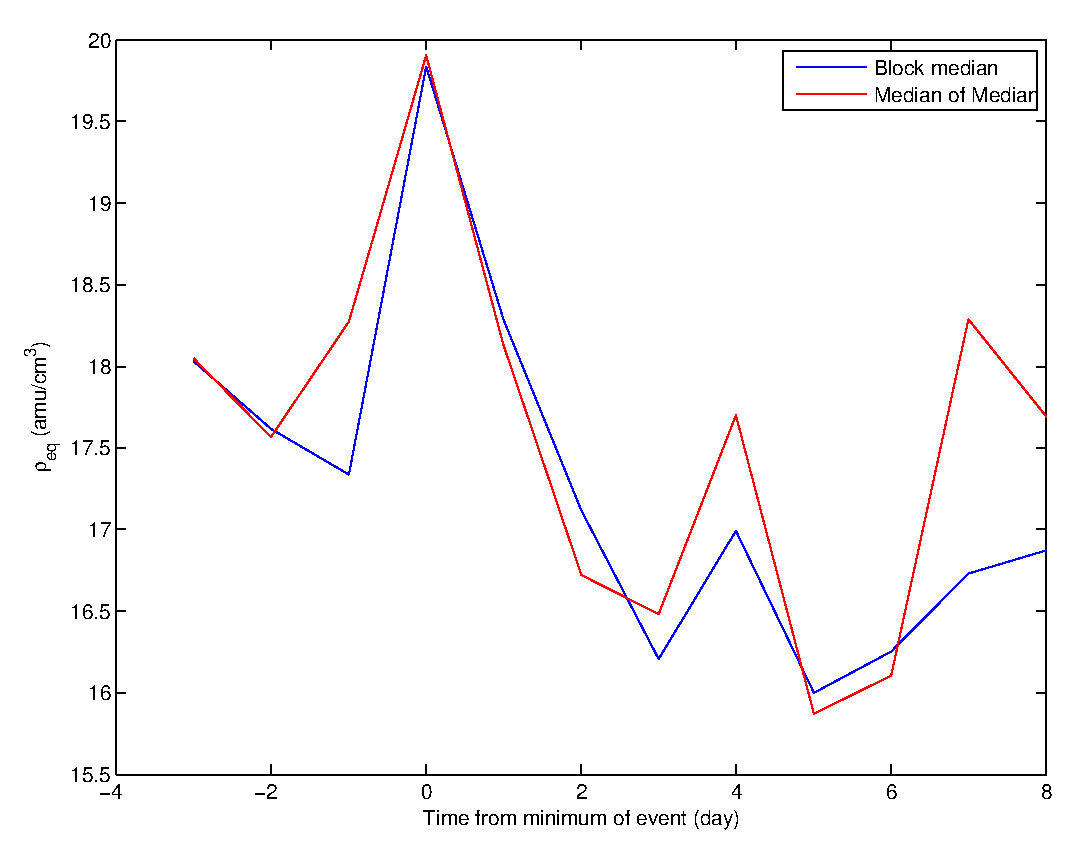
\includegraphics[scale=0.40]{paperfigures/blockmedian-prenoon.eps}
\caption{Comparing median values calculated as median of all 1-hour points in the 12 day block, and as the daily median of all hourly-mediated events. (b) Same, but only events starting between 0-12 UTC}
\label{blockmedian}
\end{figure}
\clearpage

\begin{figure}[tp]
\centering
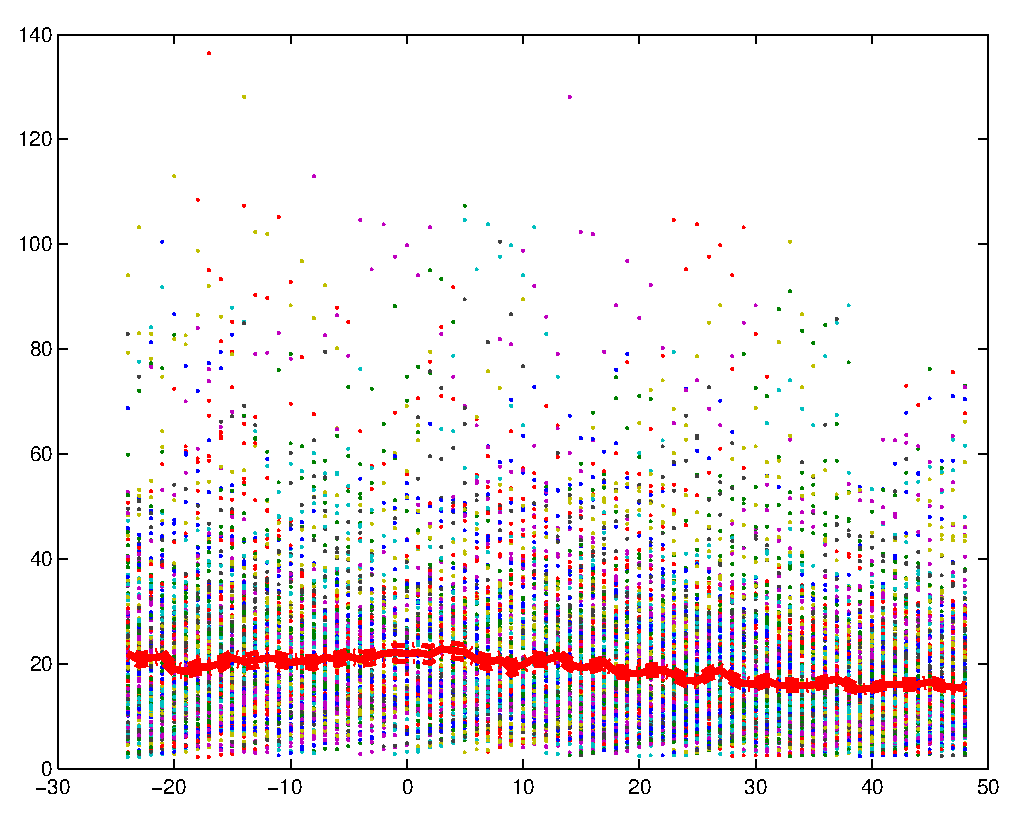
\includegraphics[scale=0.9]{paperfigures/allstorms.eps}
\caption{Comparing all events to their median and $1\sigma$ range}
\label{allstorms}
\end{figure}
\clearpage

\begin{figure}[tp]
\centering
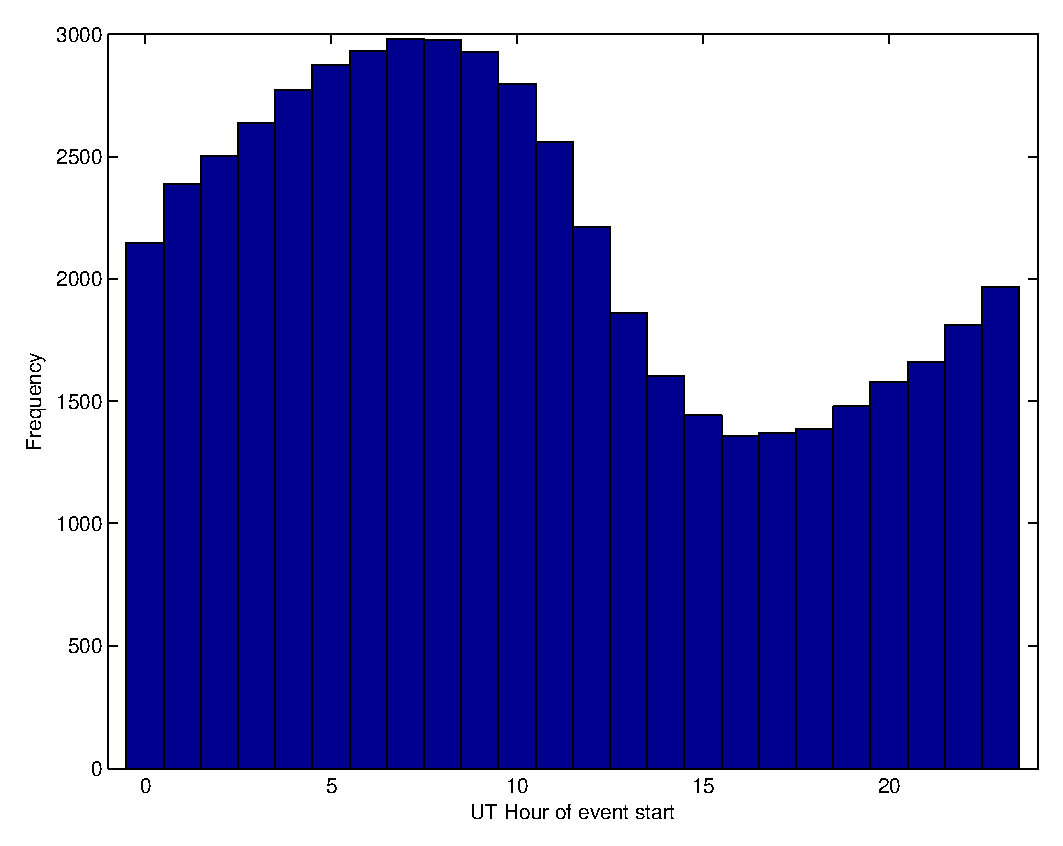
\includegraphics[scale=0.5]{paperfigures/nansbyhour.eps}
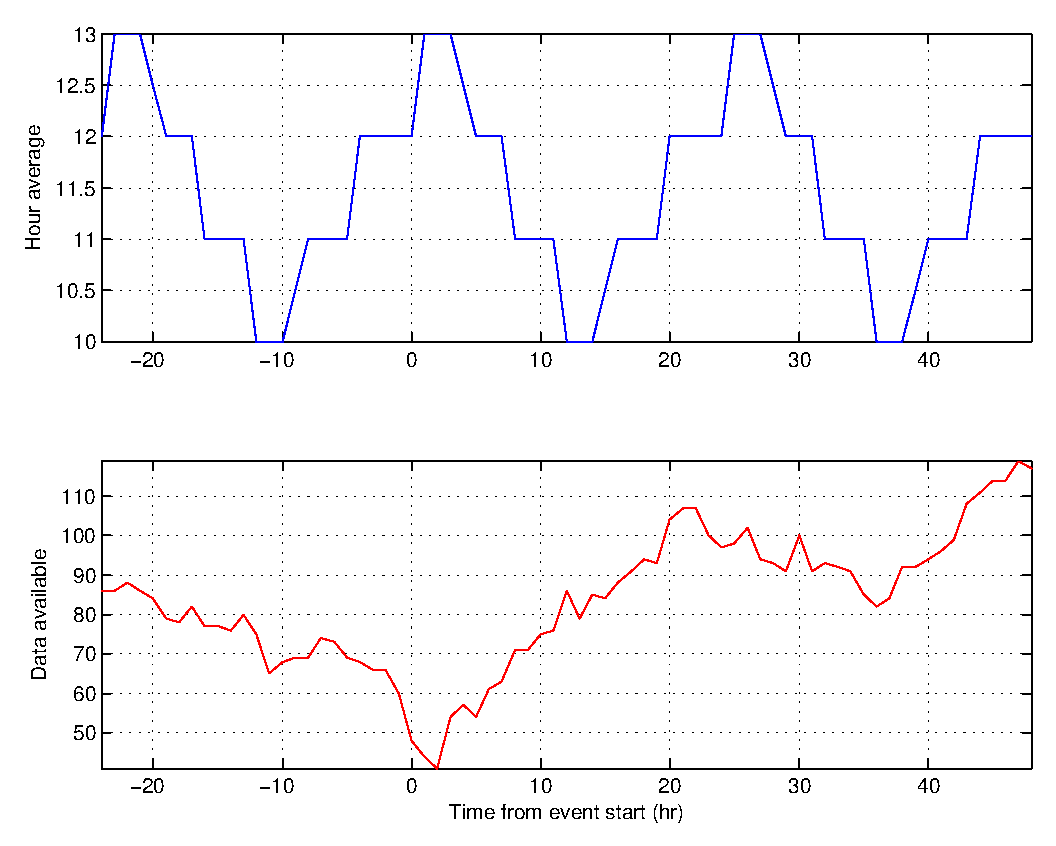
\includegraphics[scale=0.5]{paperfigures/nansbyhour_storm.eps}
\caption{(a) Number of NaN points per hour of observation in the total data set (b) $\rho_{eq}$ data availability relative to average event hour in events where $D_{st}<-80$~nT.}
\label{nanperhour}
\end{figure}
\clearpage



\section{Appendix}
\hfill
\begin{figure}[htp!]
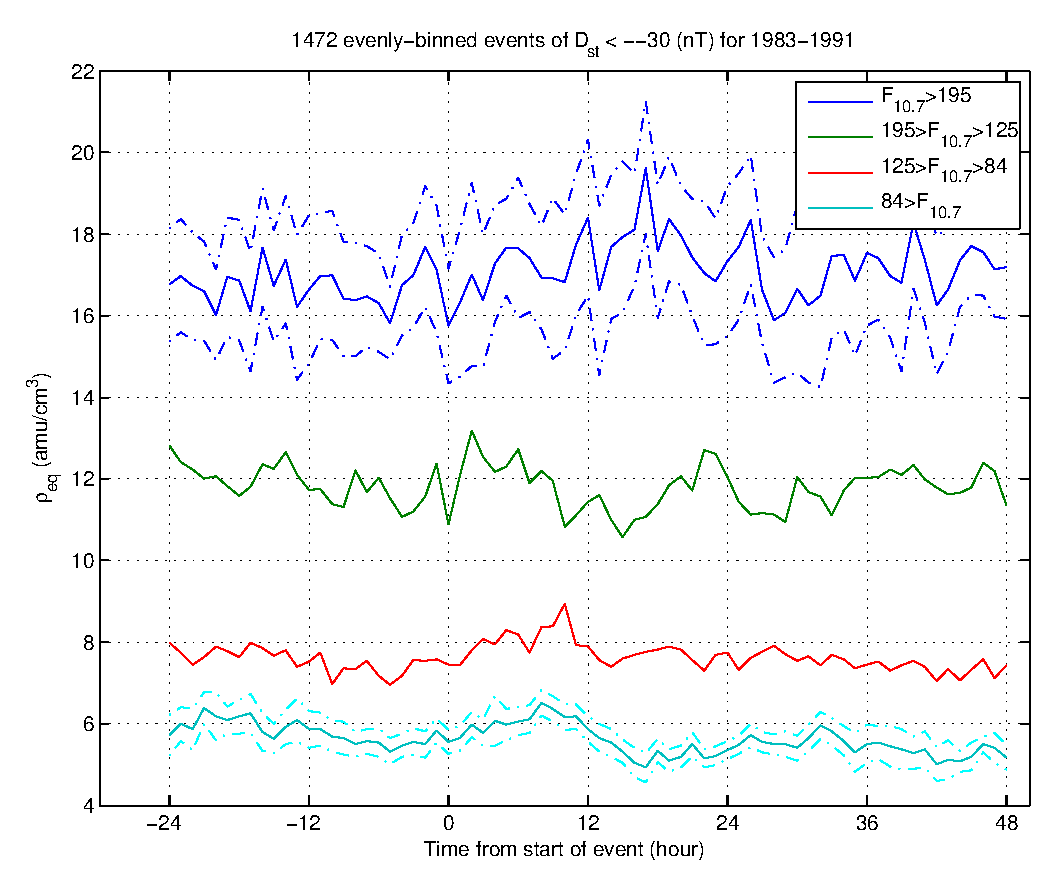
\includegraphics[scale=0.45]{paperfigures/HighLowF107rhoeq-Dst30.eps}
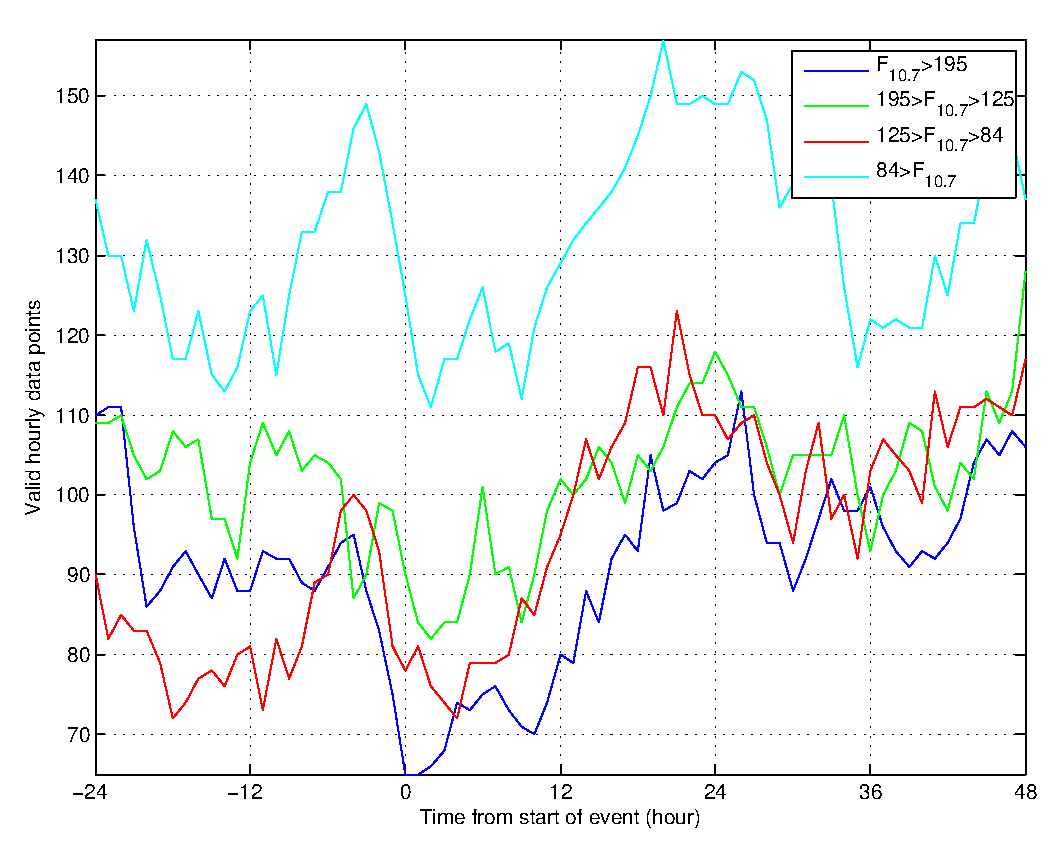
\includegraphics[scale=0.45]{paperfigures/HighLowF107rhoeq-Dst30-valid.eps}
\caption{$D_{st} < -30$ nT events, $\rho_{eq}$ binned by $F_{10.7}$. Lower panel: valid hourly points}
\end{figure}
\hfill
\begin{figure}[htp!]
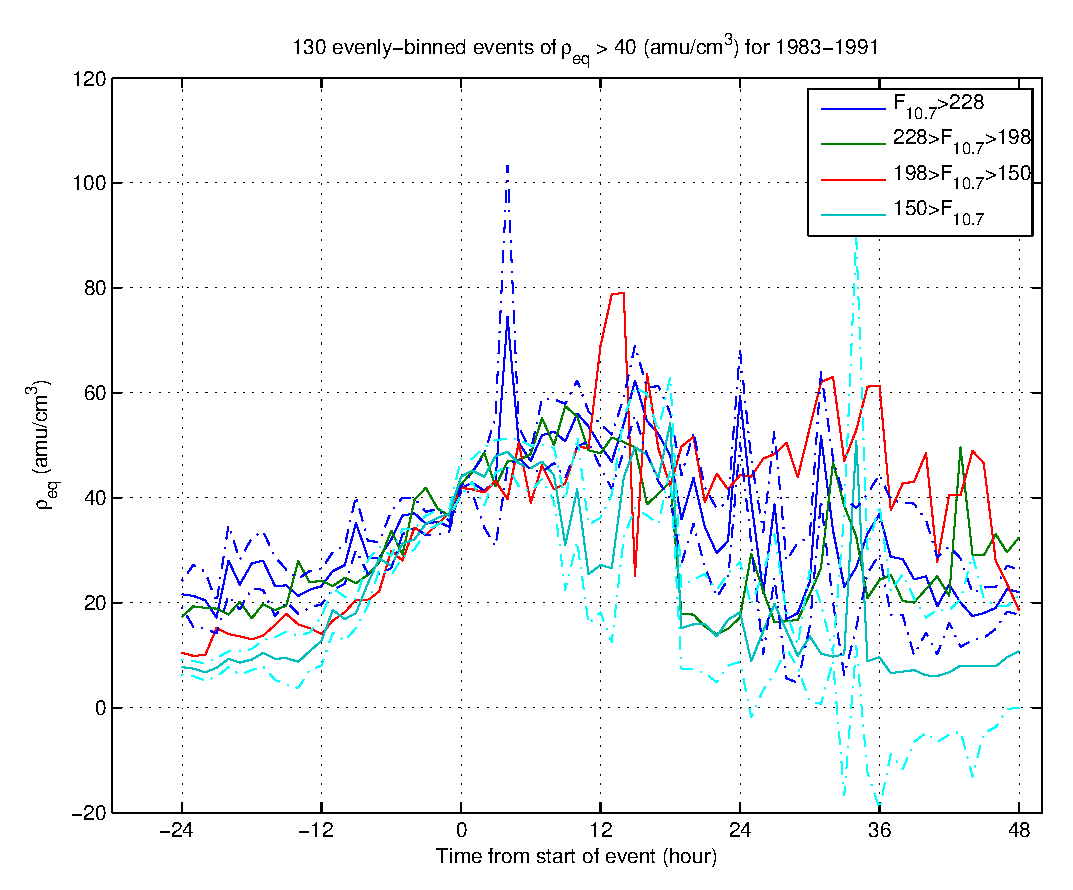
\includegraphics[scale=0.45]{paperfigures/HighLowF107rhoeq-rhoeq40.eps}
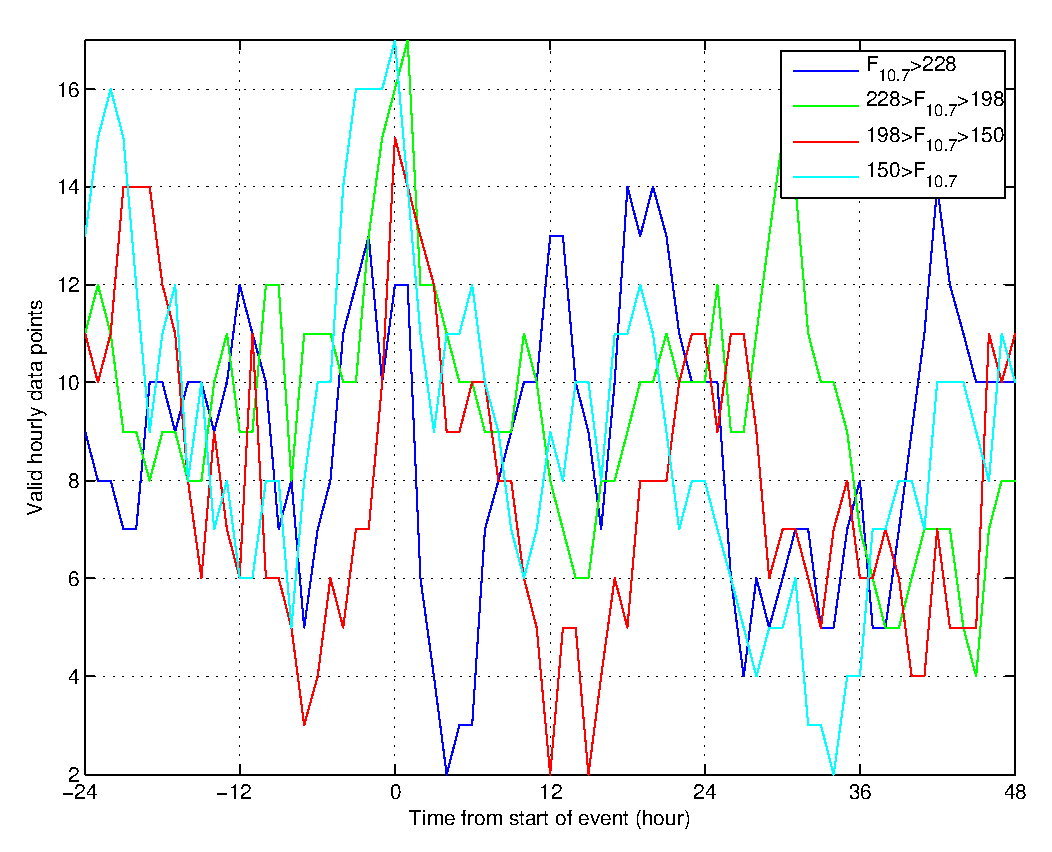
\includegraphics[scale=0.45]{paperfigures/HighLowF107rhoeq-rhoeq40-valid.eps}
\caption{$\rho_{eq} > 40$ amu/cm$^3$ events, $\rho_{eq}$ binned by $F_{10.7}$}
\end{figure}
\clearpage

\begin{figure}[htp!]
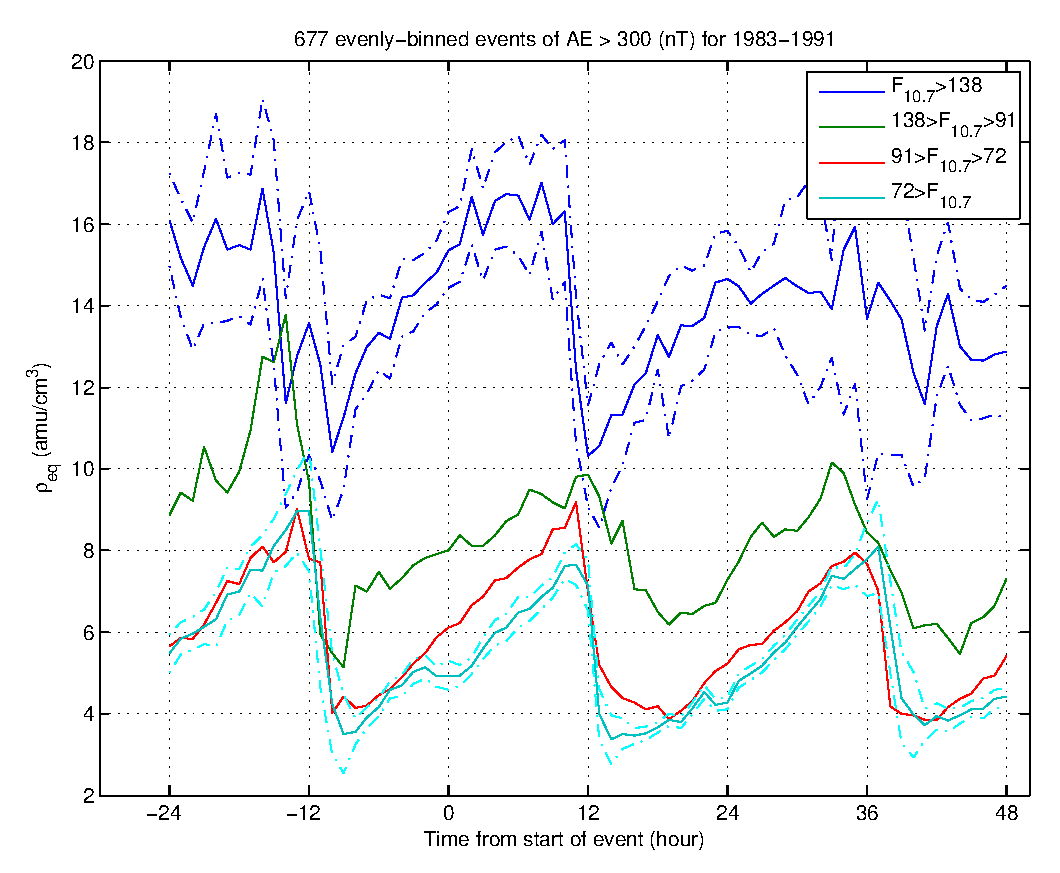
\includegraphics[scale=0.40]{paperfigures/HighLowF107rhoeq-AE300.eps}
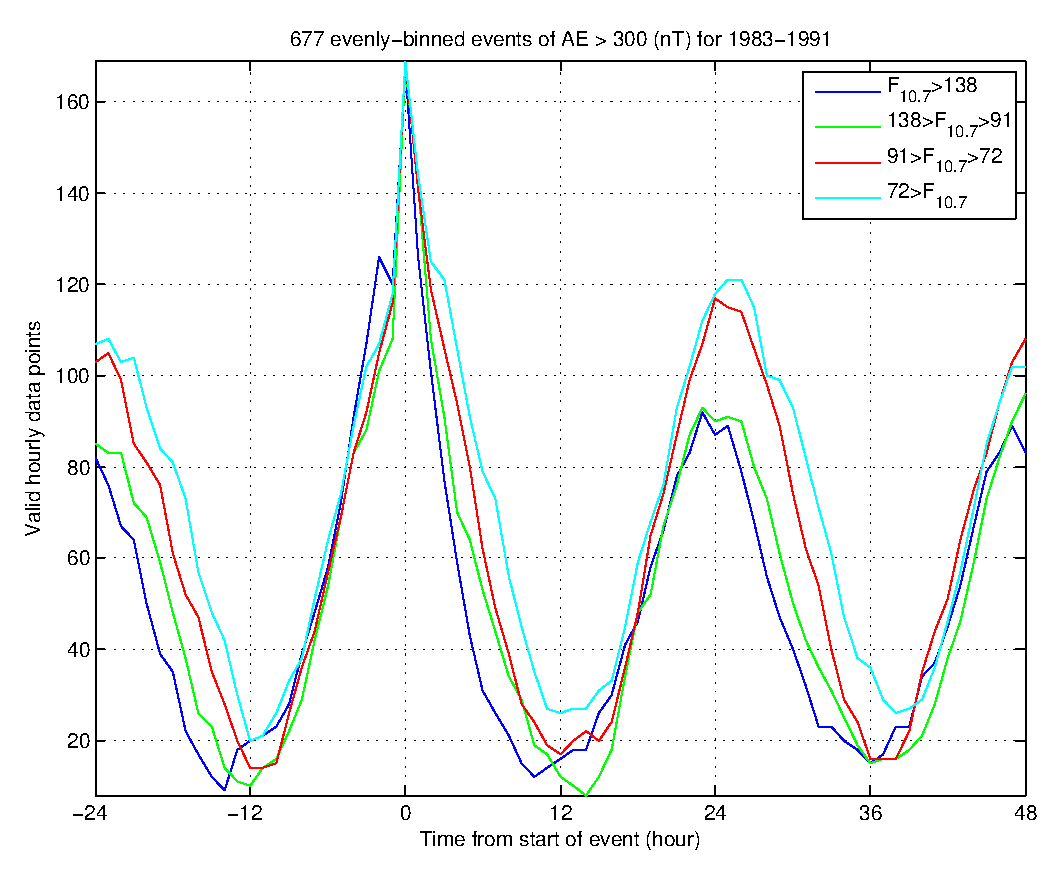
\includegraphics[scale=0.40]{paperfigures/HighLowF107rhoeq-AE300-valid.eps}
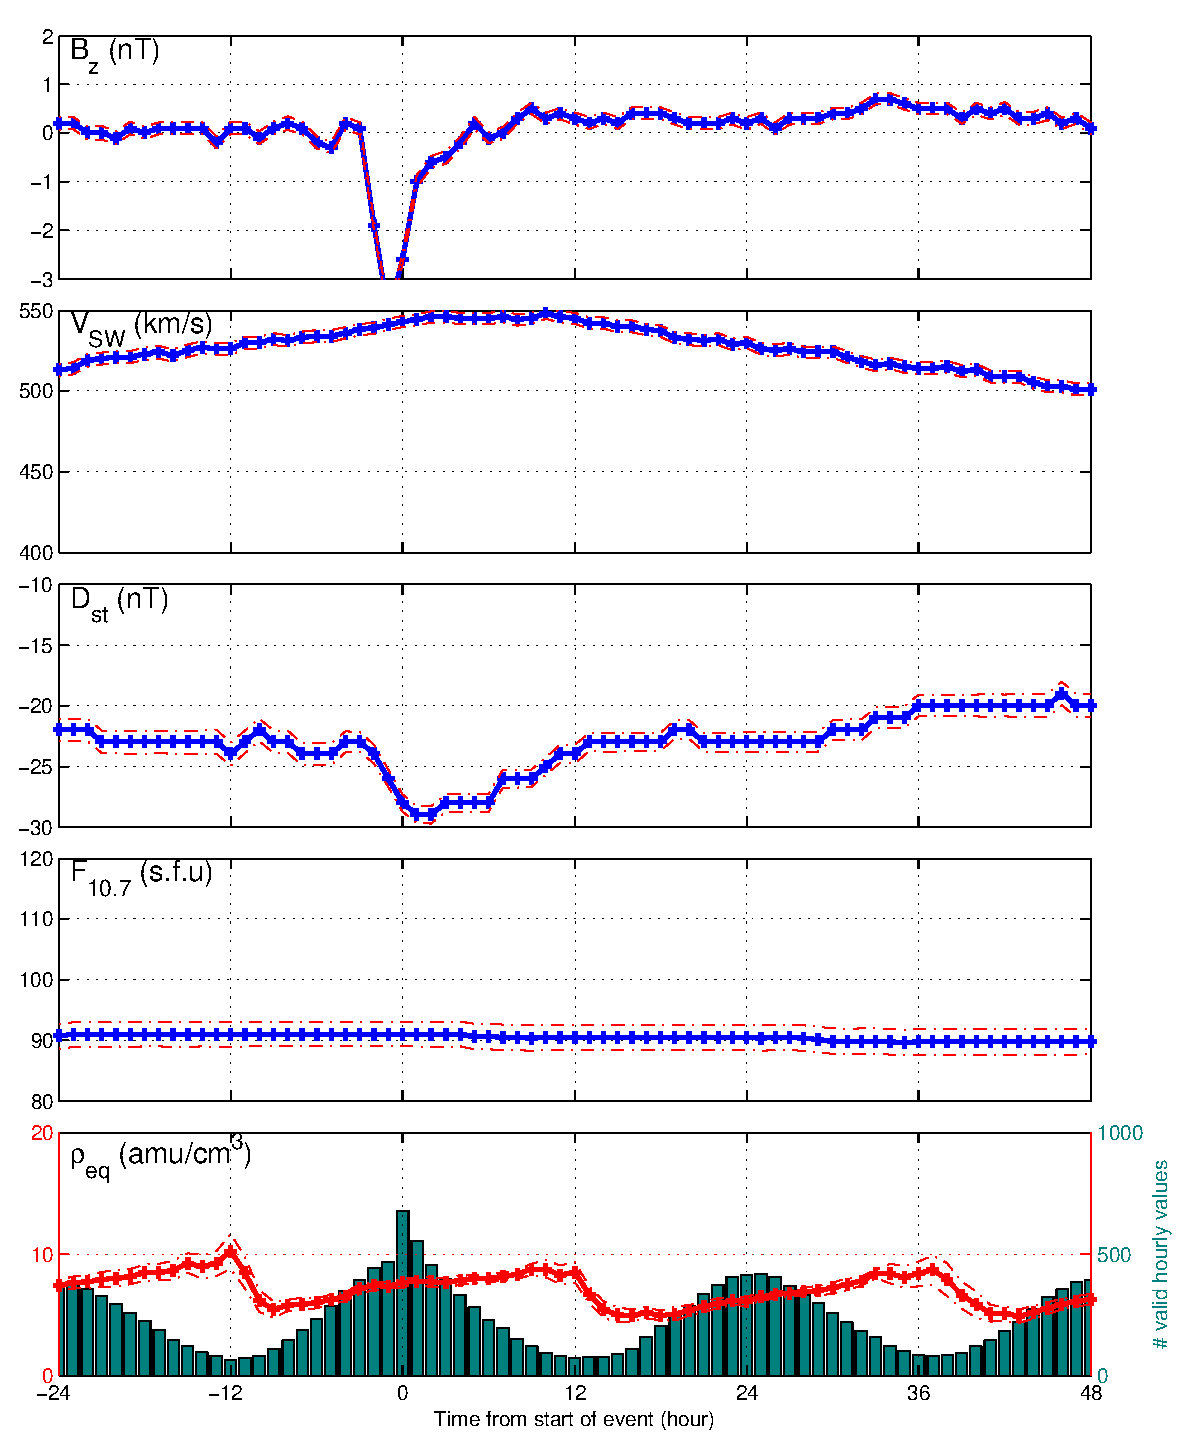
\includegraphics[scale=0.35]{paperfigures/stormavs-AE.eps}
\caption{Top: $AE > 400$ nT events, $\rho_{eq}$ binned by $F_{10.7}$ Bottom: averages of $AE > 400$ events}
\end{figure}
\hfill
\begin{figure}[htp!]
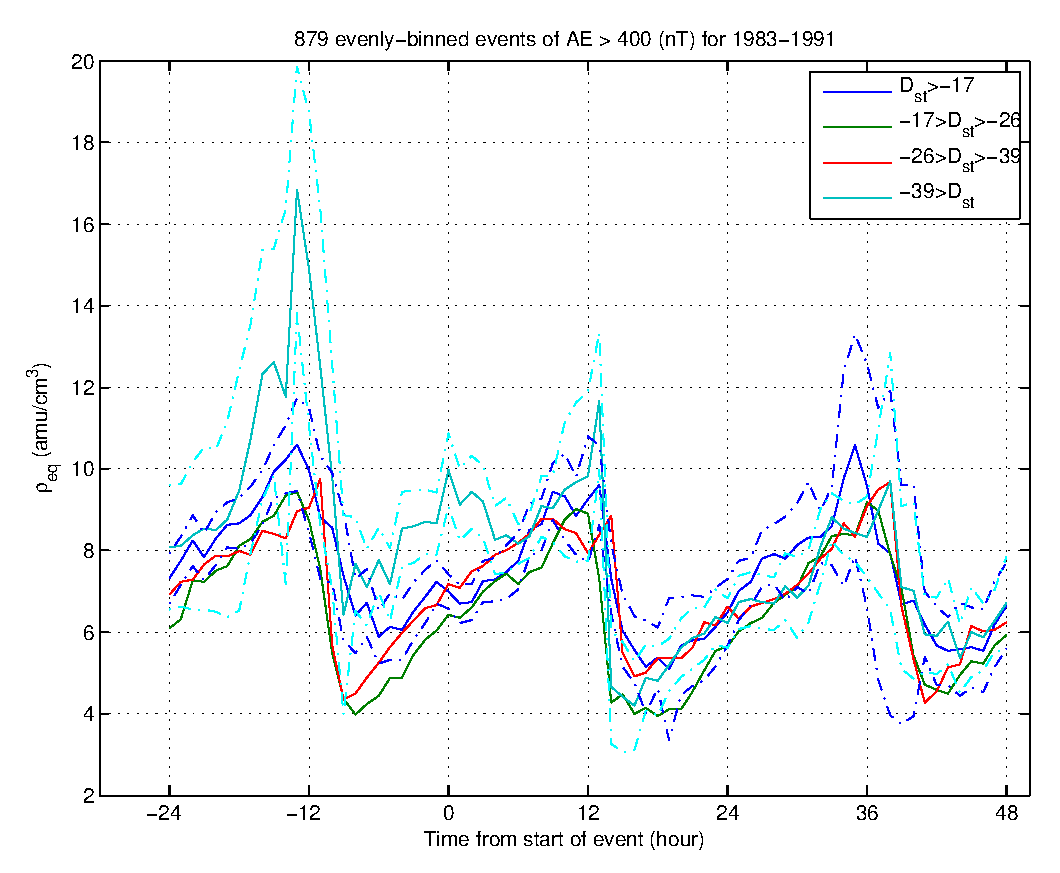
\includegraphics[scale=0.45]{paperfigures/HighLowDstrhoeq-AE400.eps}
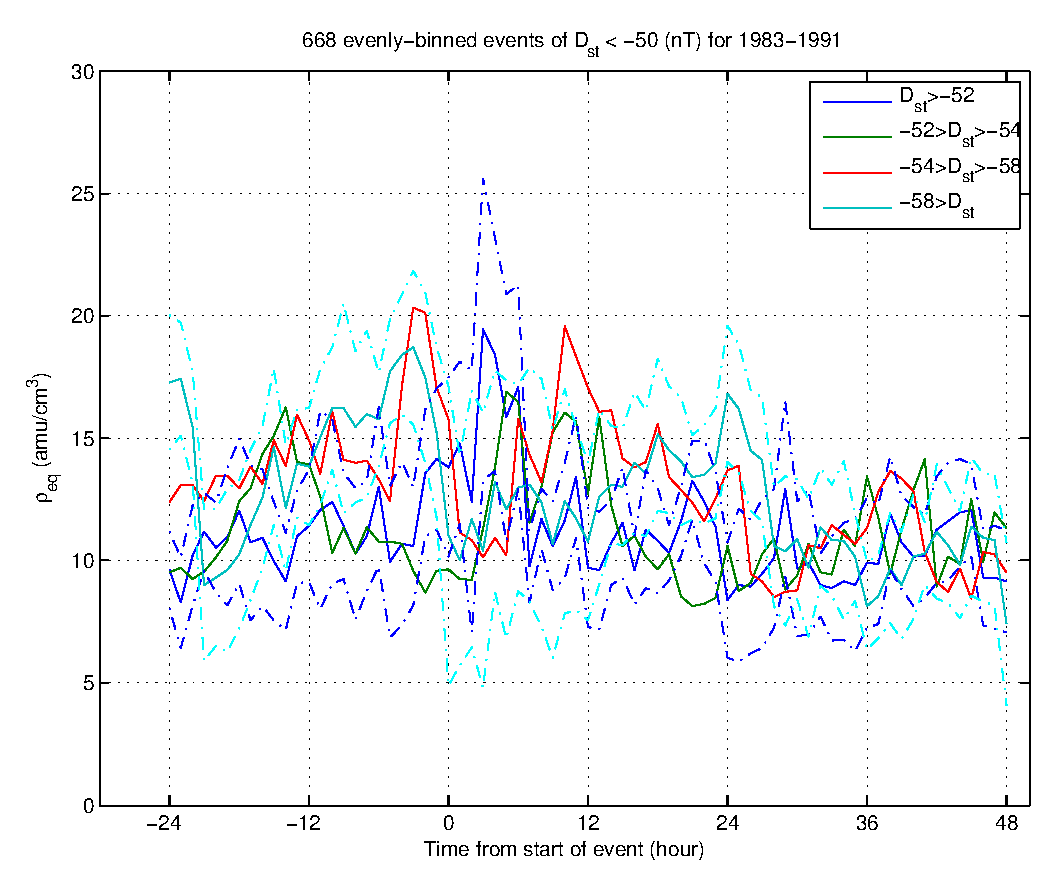
\includegraphics[scale=0.45]{paperfigures/HighLowDstrhoeq-Dst50.eps}
\caption{Top: $AE > 400$ nT events. Bottom: $D_{st} < -50$ nT events. Both $\rho_{eq}$ binned by $D_{st}$.}
\end{figure}
\clearpage

\begin{figure}[htp!]
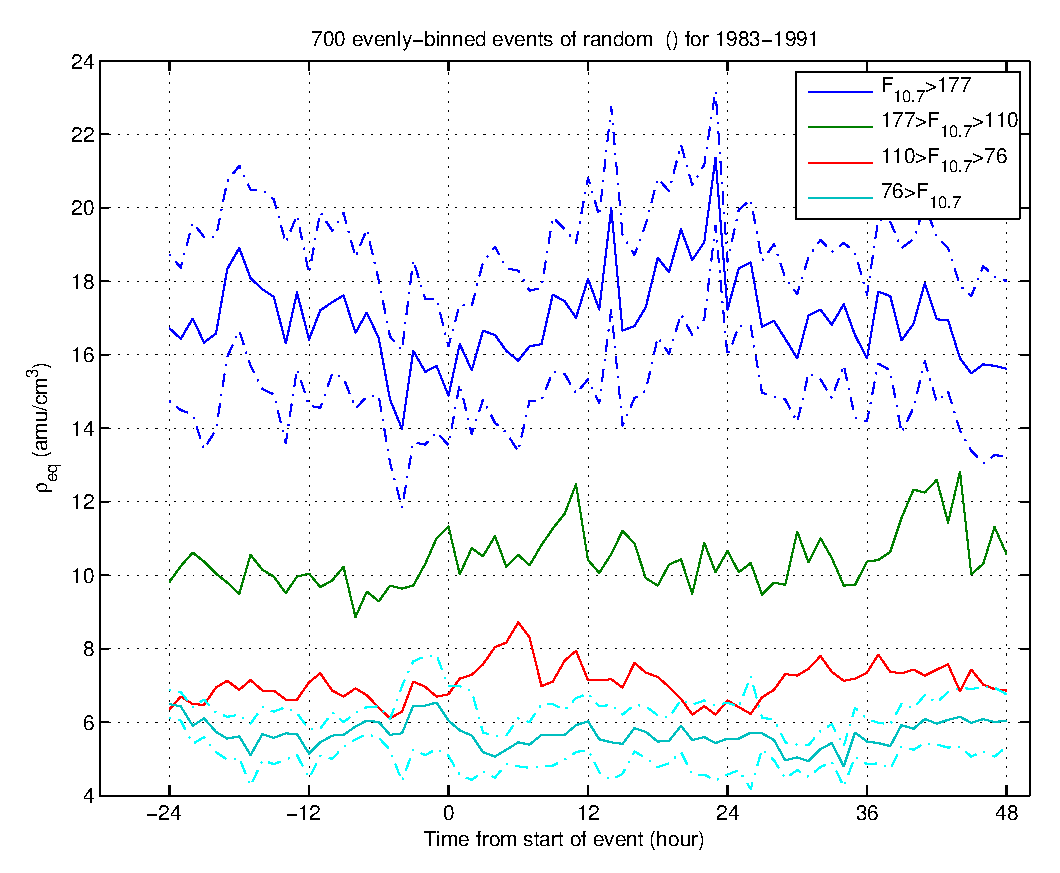
\includegraphics[scale=0.45]{paperfigures/HighLowF107rhoeq-random.eps}
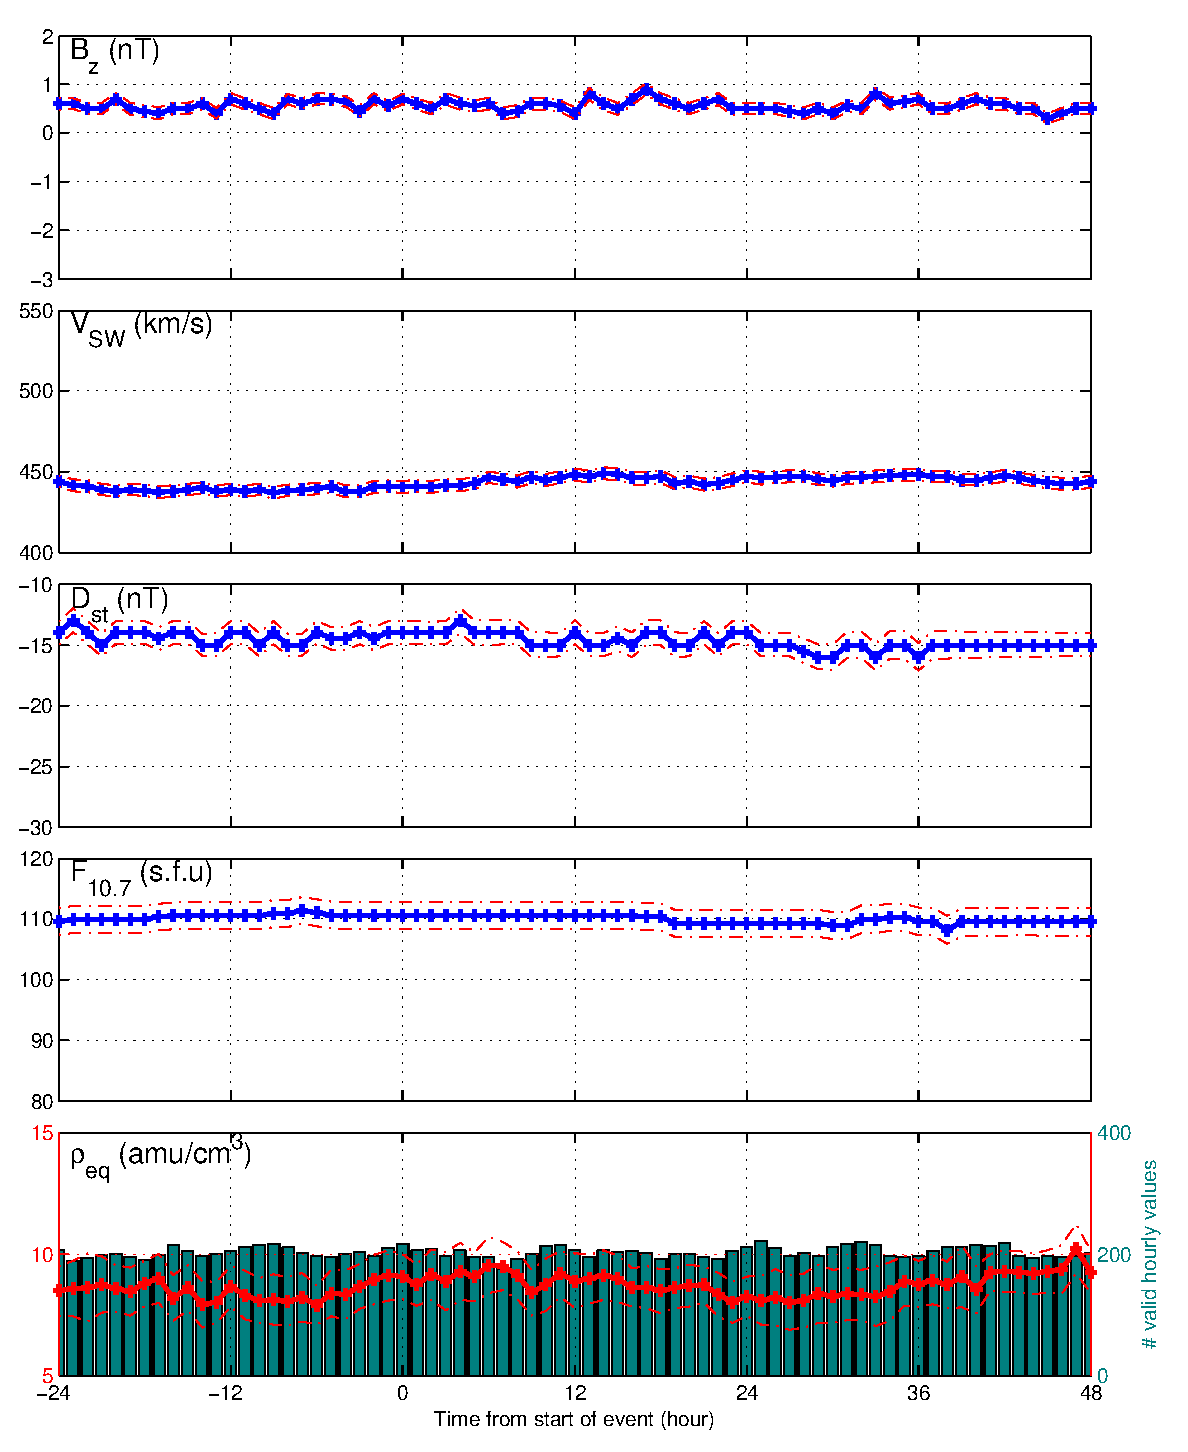
\includegraphics[scale=0.45]{paperfigures/stormavs-random.eps}
\caption{Top: $\rho_{eq}$ binned by $F_{10.7}$ for randomly selected times. Bottom: averages of randomly selected times}
\end{figure}

\begin{figure}[htp!]
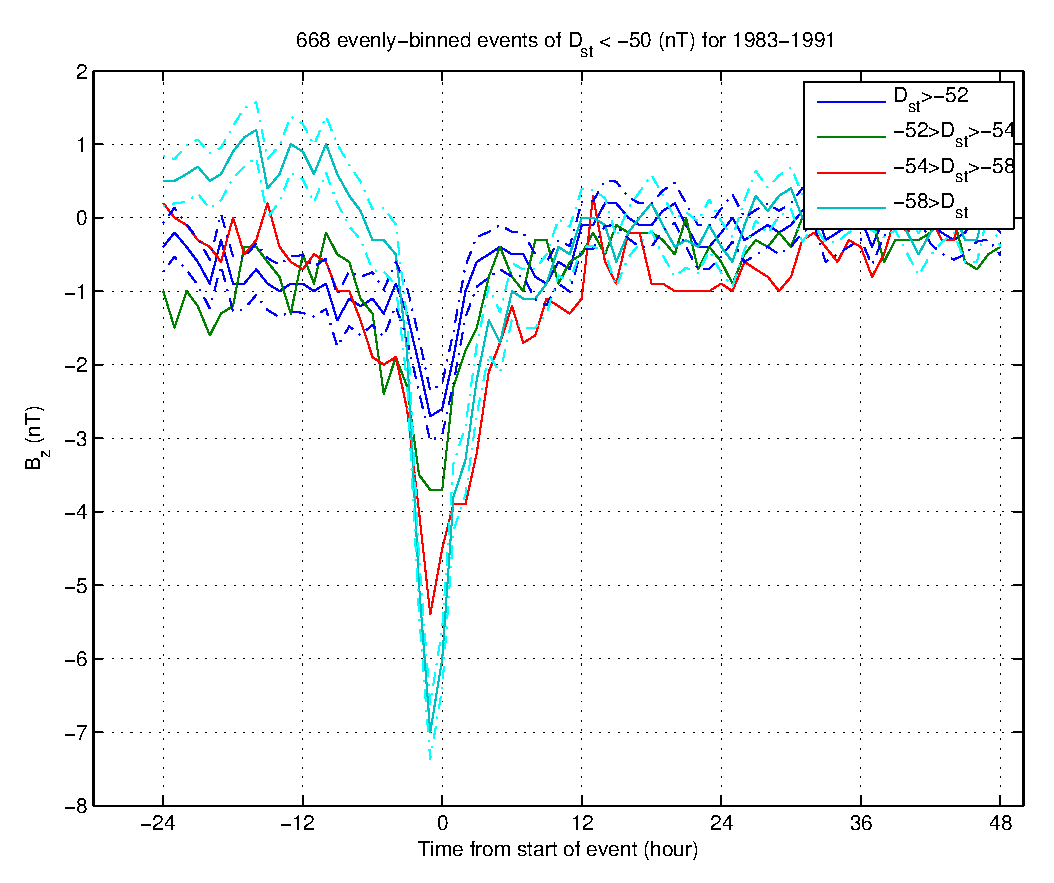
\includegraphics[scale=0.45]{paperfigures/HighLowDstBz-Dst50.eps}
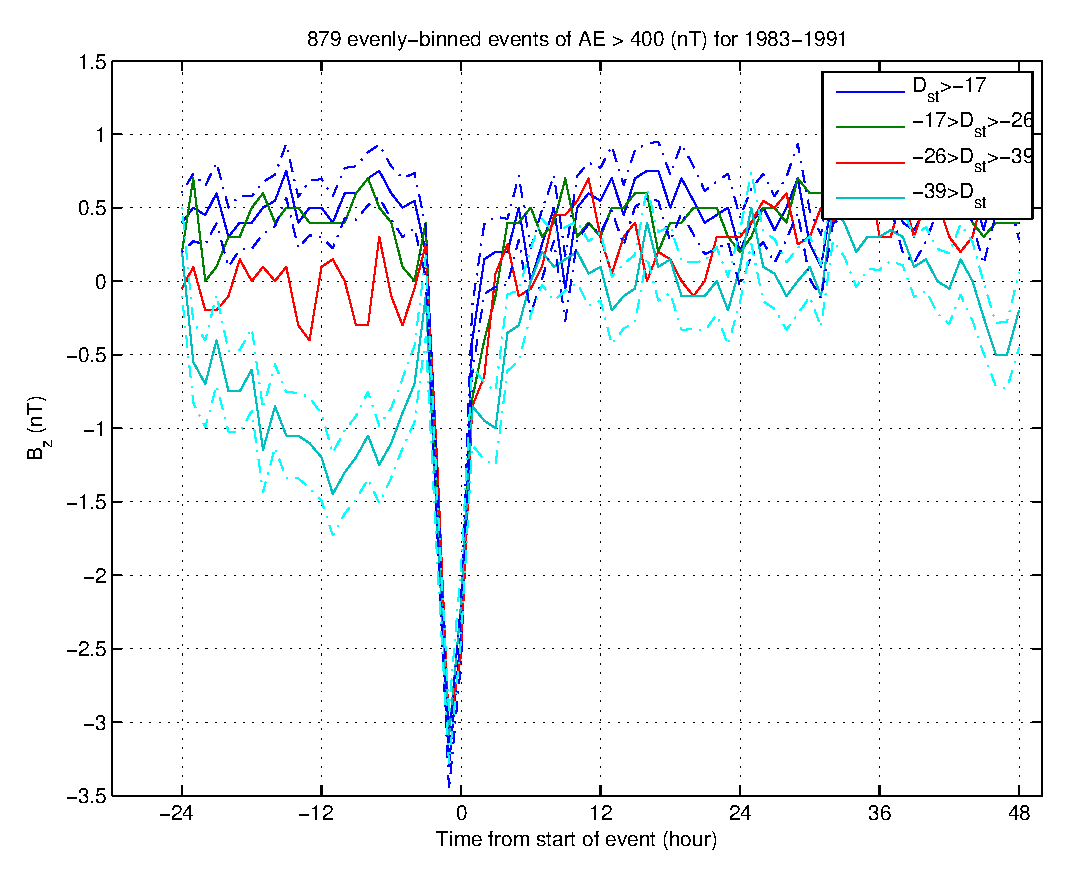
\includegraphics[scale=0.45]{paperfigures/HighLowDstBz-AE400.eps}
\caption{Top: $B_z$ binned by $D_{st}$ for $D_{st} < -50$ nT events. Bottom: $B_z$ binned by $D_{st}$ for $AE > 400$ nT events}
\end{figure}
\clearpage

\begin{figure}[htp!]
\includegraphics[scale=0.45]{paperfigures/rhoMLT.eps}
\includegraphics[scale=0.45]{paperfigures/rhoLT.eps}
\caption{Median $\rho_{eq}$ vs magnetic local time and universal time}
\end{figure}

\begin{figure}[htp!]
\includegraphics[scale=0.45]{paperfigures/DstLT.eps}
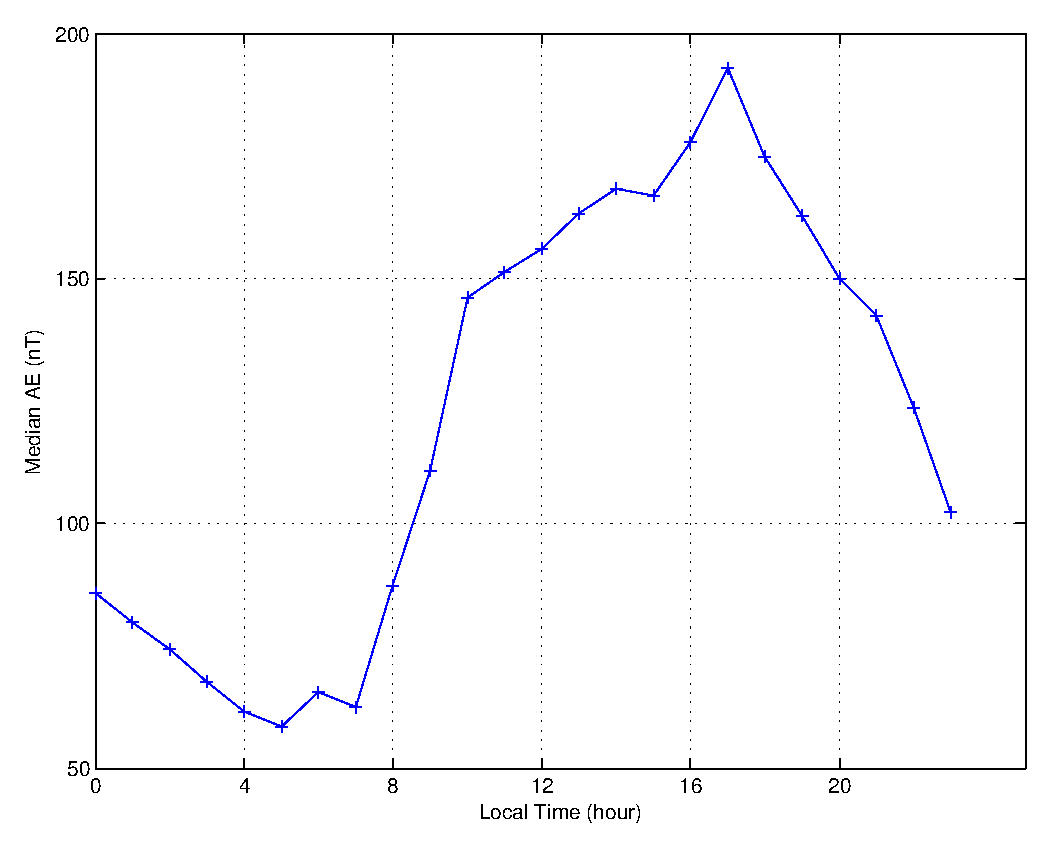
\includegraphics[scale=0.45]{paperfigures/AELT.eps}
\caption{Median $D_{st}$ vs universal time, and median AE vs universal time}
\end{figure}
\clearpage


\begin{figure}[htp!]
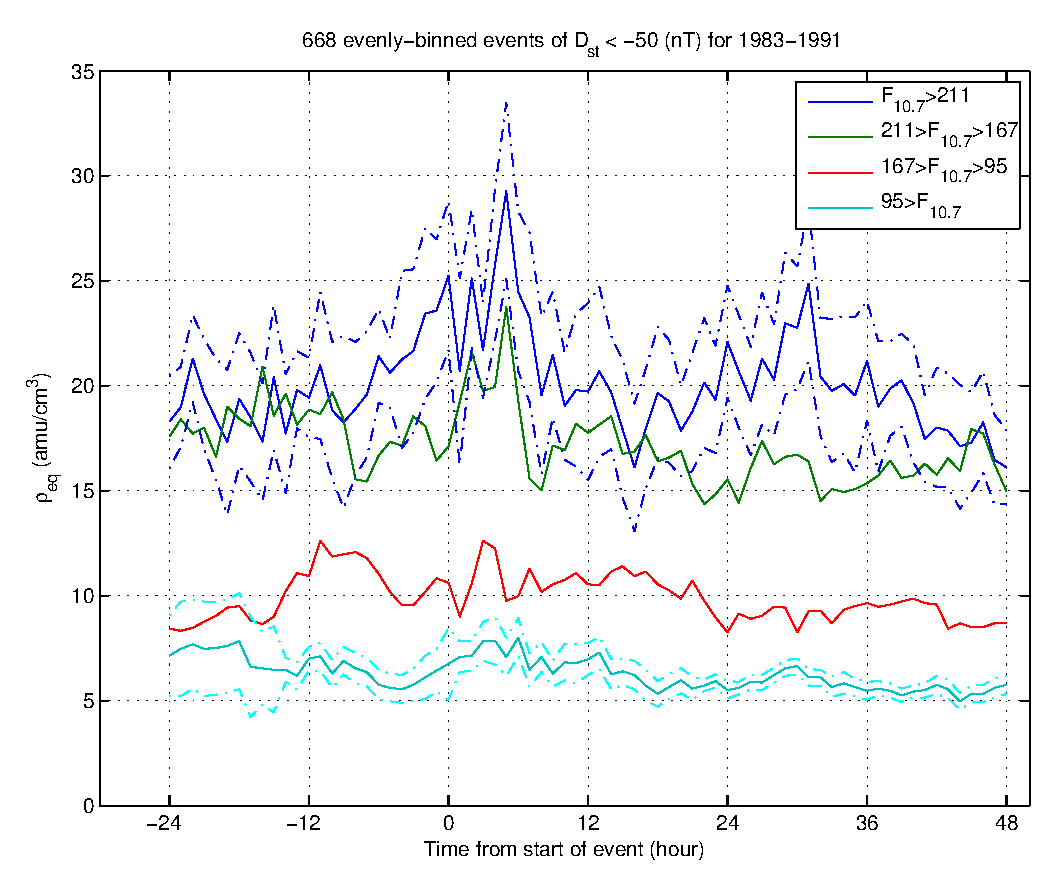
\includegraphics[scale=0.45]{paperfigures/HighLowF107rhoeq-Dst50-sat6.eps}
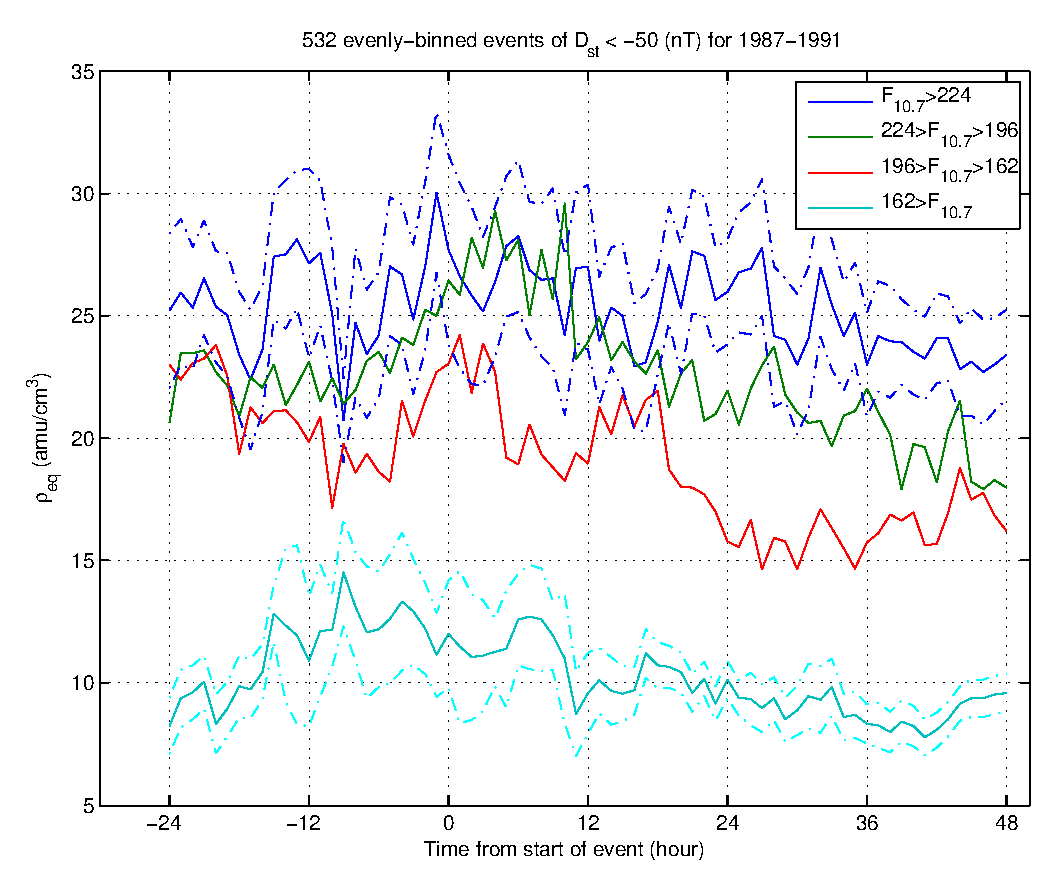
\includegraphics[scale=0.45]{paperfigures/HighLowF107rhoeq-Dst50-sat7.eps}
\caption{GOES Satellite 6 and 7}
\end{figure}

\begin{figure}[htp!]
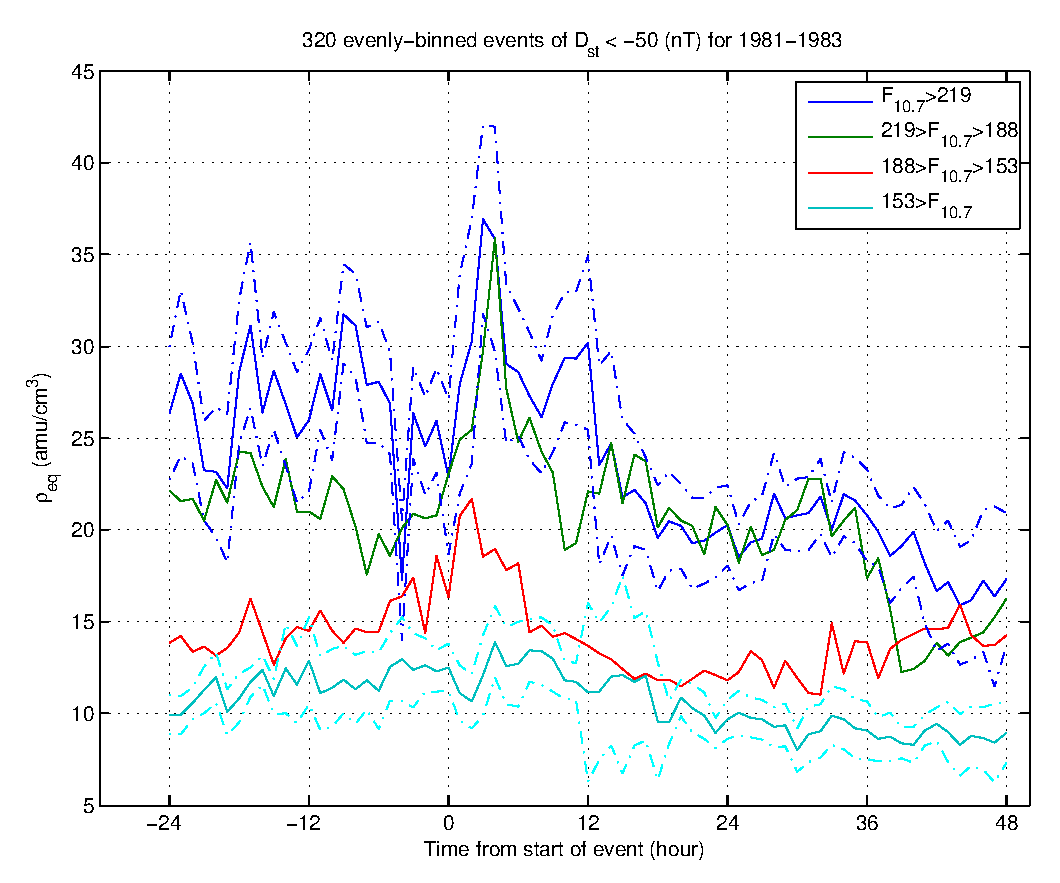
\includegraphics[scale=0.45]{paperfigures/HighLowF107rhoeq-Dst50-sat2.eps}
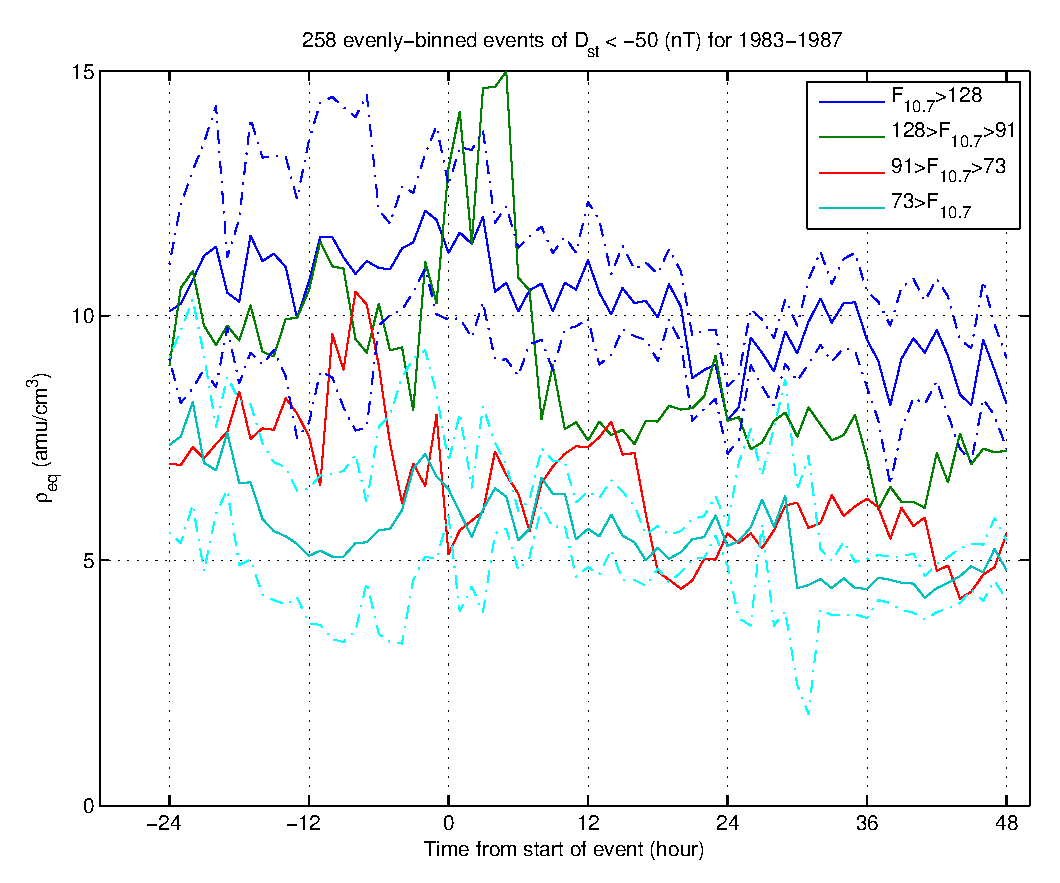
\includegraphics[scale=0.45]{paperfigures/HighLowF107rhoeq-Dst50-sat5.eps}
\caption{GOES Satellite 2 and 5}
\end{figure}
\clearpage

\begin{figure}[htp!]
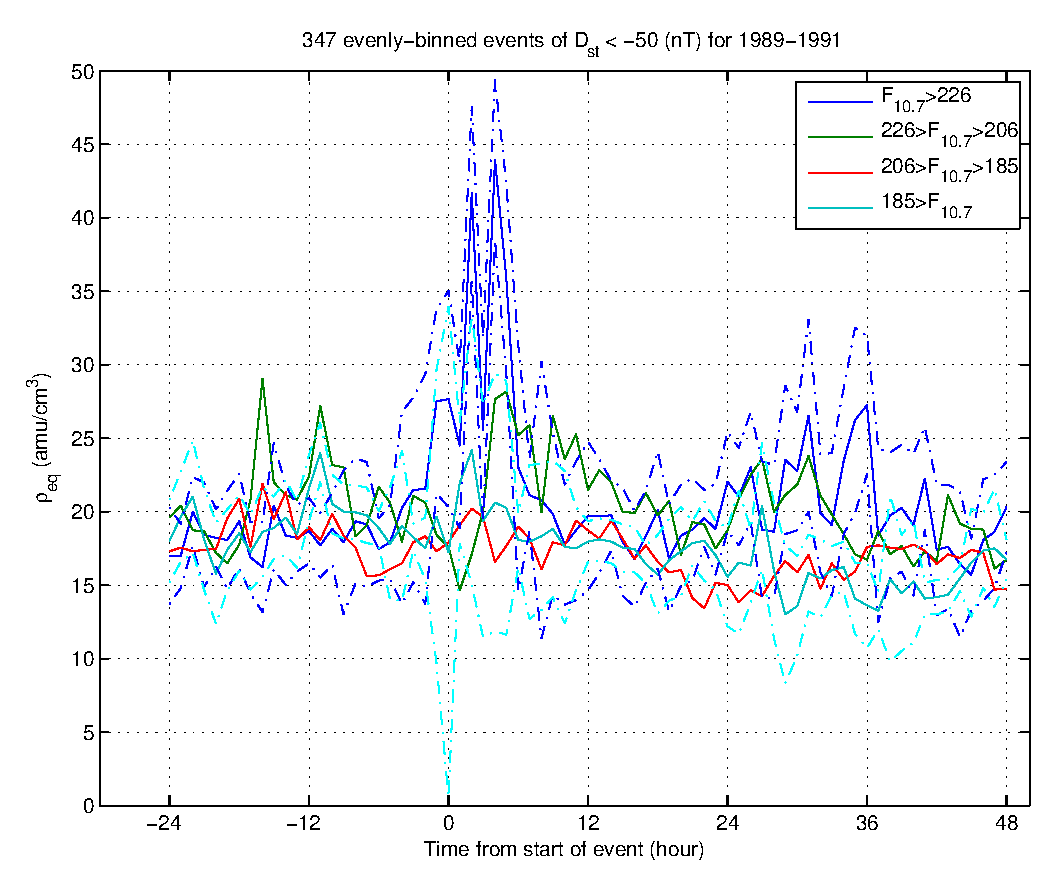
\includegraphics[scale=0.45]{paperfigures/HighLowF107rhoeq-Dst50-tak.eps}
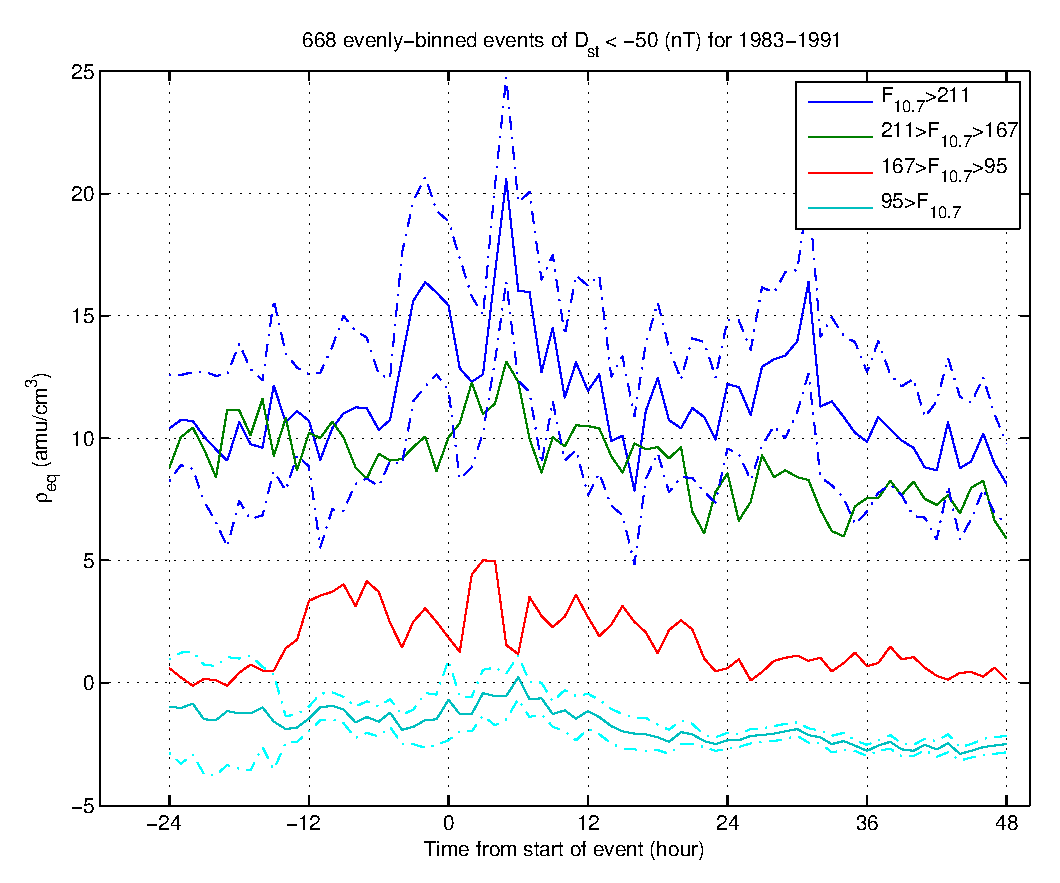
\includegraphics[scale=0.45]{paperfigures/HighLowF107rhoeq-Dst50-detrend.eps}
\caption{Top: From 89-91. Bottom: With $\rho_{eq}$ LT medians subtracted}
\end{figure}

\begin{figure}[htp!]
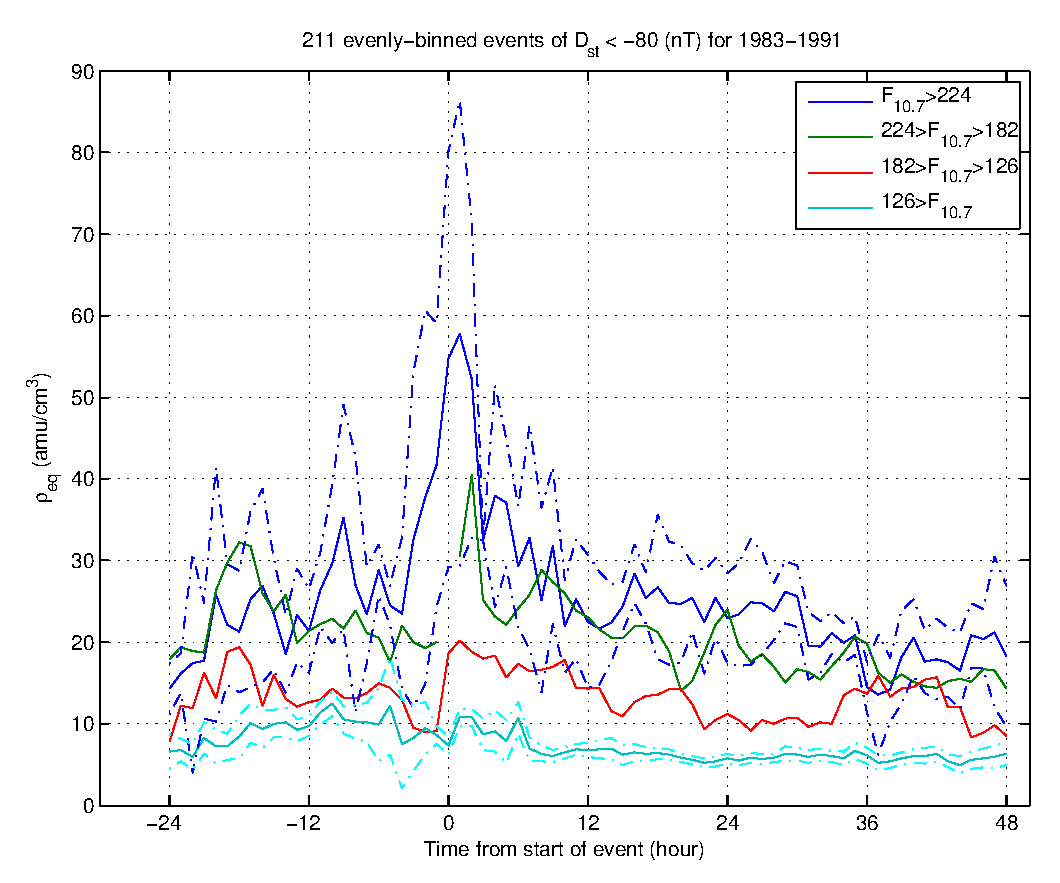
\includegraphics[scale=0.45]{paperfigures/HighLowF107rhoeq-Dst80.eps}
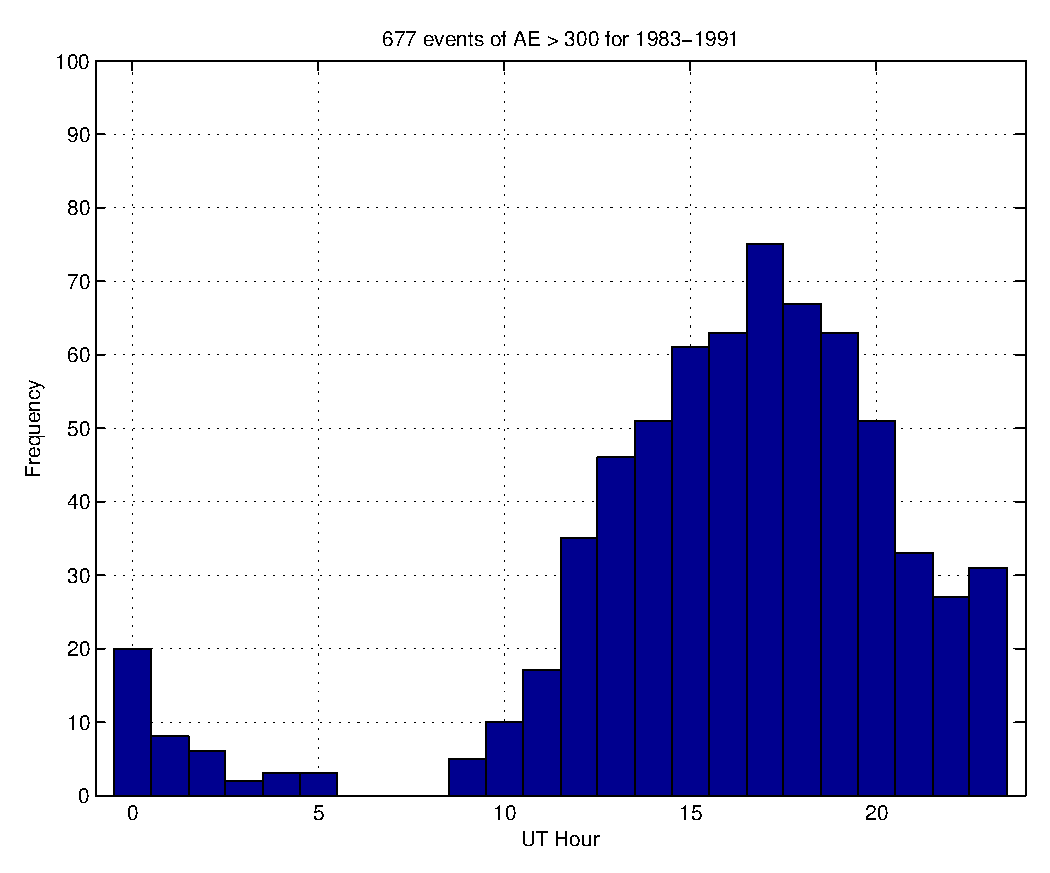
\includegraphics[scale=0.45]{paperfigures/AEbyhour.eps}
\caption{Top: $D_{st}<-80$~nT. Bottom: $AE$ events by their hour of onset}
\end{figure}
\clearpage

\begin{figure}[htp!]
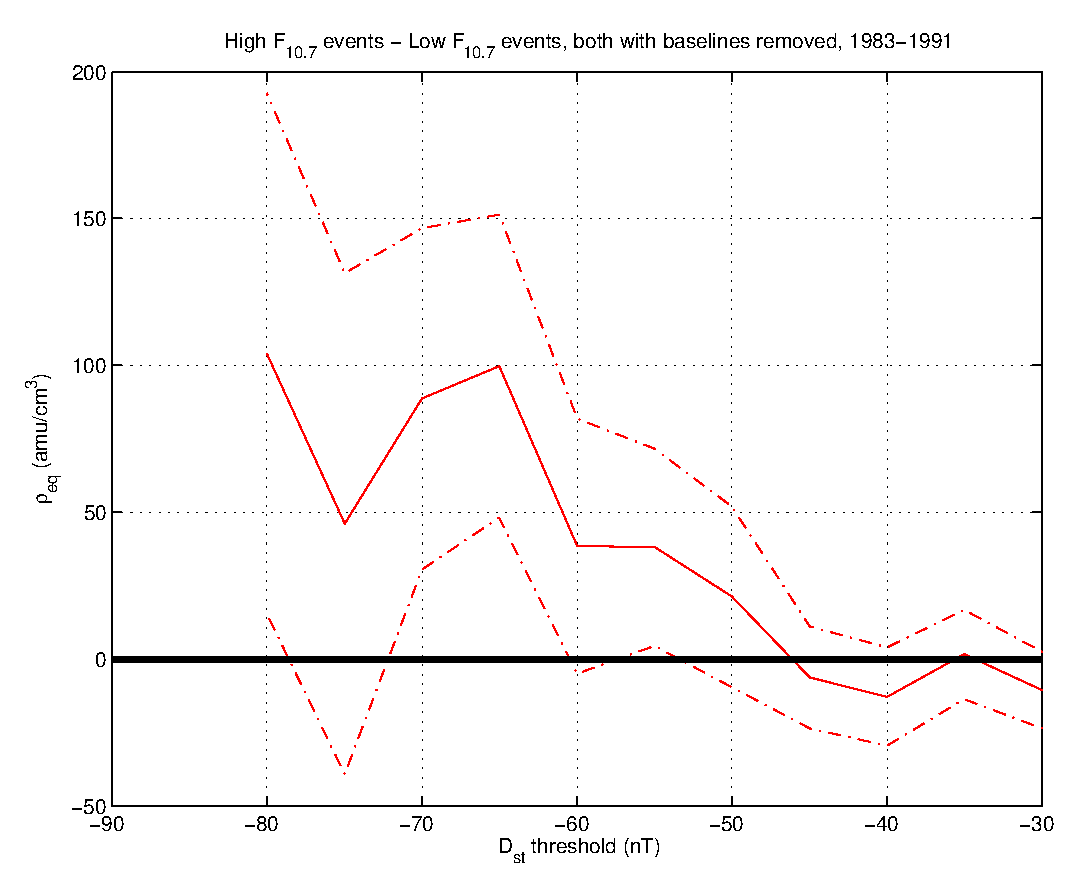
\includegraphics[scale=0.45]{paperfigures/DstRhoThresh-1983-1991.eps}
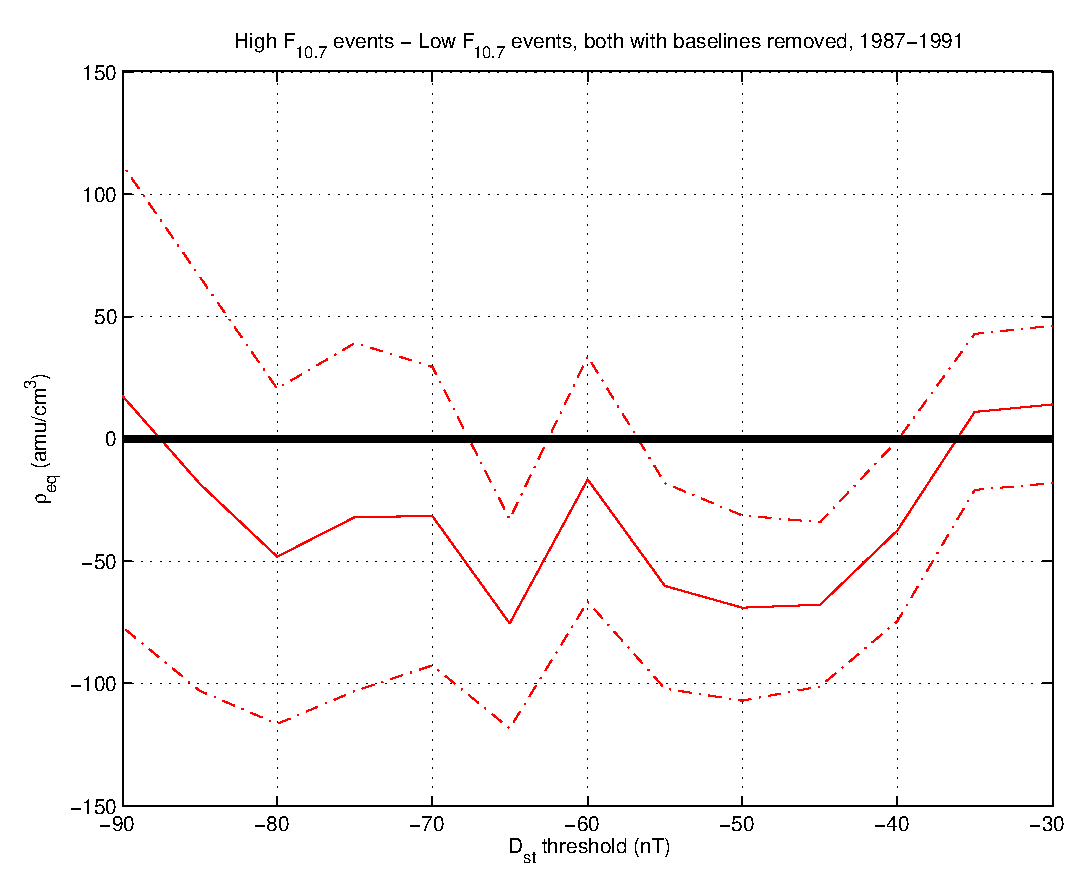
\includegraphics[scale=0.45]{paperfigures/DstRhoThresh-1987-1991.eps}
\caption{High $F_{10.7}$ events - Low $F_{10.7}$ events, both with baselines removed. 83-91 and 87-91}
\end{figure}

\begin{figure}[htp!]
\includegraphics[scale=0.45]{paperfigures/DstRhoThresh-1983-1987.eps}
\includegraphics[scale=0.45]{paperfigures/DstRhoThresh-1981-1983.eps}
\caption{High $F_{10.7}$ events - Low $F_{10.7}$ events, both with baselines removed. 83-87 and 81-83}
\end{figure}


\end{document}
